\documentclass[11pt,a4paper]{book} 	% Basisdokumentenklasse
\usepackage[english]{babel}        	% Deutsche Standardbezeichner und Trennung
\usepackage[utf8]{inputenc}      
\usepackage[T1]{fontenc}          	% und {\ss}
\usepackage{makeidx}               	% Indexpaket
\usepackage{times}                 	% Schönere Schriften, Achtung, nicht pslatex verwenden!
\usepackage{longtable}             	% Lange Tabelle für Abkürzungsverzeichnis
\usepackage{graphics}              	% EPS-Grafiken einbinden
\usepackage{hyperref}
\usepackage{fancyvrb}              	% Fancy-Verbatin für Programmlistings
\usepackage{pdfpages}
\usepackage{graphicx}
\usepackage{hyperref}

\usepackage{tabularx}
\usepackage{booktabs}



\setlength{\textfloatsep}{6pt plus 2.0pt minus 4.0pt}


\usepackage{listings}			  	% For code snippet
\usepackage{color}
\definecolor{commentgray}{HTML}{8C8C8C}
\definecolor{stringgreen}{HTML}{077D16}
\definecolor{keywordorange}{HTML}{CB7832}
\definecolor{constantpurple}{HTML}{92268F}
\lstset{frame=tb,
  language=Java,
  aboveskip=3mm,
  belowskip=3mm,
  showstringspaces=false,
  columns=flexible,
  basicstyle={\small\ttfamily},
  numbers=none,
  numberstyle=\tiny\color{black},
  keywordstyle=\color{keywordorange},
  commentstyle=\color{commentgray},
  stringstyle=\color{stringgreen},
  breaklines=true,
  breakatwhitespace=true,
  morecomment=[s][\color{constantpurple}] {trainingDataSiz}{e},
  morecomment=[s][\color{constantpurple}] {predictionHorizo}{n},
  morecomment=[s][\color{constantpurple}] {windowSiz}{e},
  tabsize=3,
  numbers=left
}


\usepackage{abtmobithesis/abtmobithesis}           % Das Abteilungs-Stylepaket, am Ende einbinden!


% Settings for title page
\title{Balancing Performance and \\[-0.2em]Resource-Awareness:\\[0.6em] Optimizing the Model Selection and Ensemble Process in Machine Learning}
\author{Niklas Diller}
\date{\today}
\studiengang{Master’s Degree in Computing in the Humanities}
\arbeitstyp{Master's  Thesis}
\erstgutachter{Prof. Dr. Daniela Nicklas}
\zweitgutachter{Michael Freitag}

% Index erneuern
\makeindex

% Das eigentliche Dokument
\begin{document}


% Anfang des Dokuments
\maketitle              % Title page

\newpage
\thispagestyle{empty}
\cleardoublepage

\pagenumbering{Roman}   

% TODO Abstract
\chapter*{Abstract}
 
 
 Accomplishing an appropriate trade-off between a machine learning model's performance and resource awareness is a challenge that increasingly necessitates the attention of data scientists and engineers, especially in edge computing. Ensuring that a certain deployed model efficiently utilizes its resources is crucial for minimizing battery consumption, managing computational resources, and freeing up network bandwidth. Particularly when working with large model databases, it can prove to be rather cumbersome to select models that fulfill this requirement in addition to providing accurate predictions. This task only gets more complex when working with sets of different models, as the number of possible model combinations exponentially increases the more learners are considered for set creation.
  
 Largely motivated by current research projects in cattle activity recognition and parking availability prediction, this work explores approaches to balance performance and resource awareness in the model selection process and introduces a model set retrieval system that allows for detailed customizable settings in a multi-object optimization context. After presenting essential theoretical concepts about the top-k algorithms Fagin's Algorithm (FA) \cite{fagin1999} and Threshold Algorithm (TA) \cite{fagin2002a}, a paradigm of different scores is constructed that aims to depict the performance and resource awareness of a model set concurrently and precisely. 
 
  For the retrieval system to work on actual objects, a large number of models have been trained and stored by using a preprocessing and training pipeline that was developed for this work. The user is then given the option to choose one of three top-k algorithms amongst several other settings to have a model set based on their preferences returned to them. To assess resource awareness in the model sets, the concept is split up into intra- and inter-model resource awareness. While the extent of efficient resource utilization among multiple models is measured by ascertaining commonalities between them using Query Sharing Levels (QSLs), single-model metrics like the number of features a model was trained on or its window size are used as a first indicator for a model's resource awareness. This distinction between intra- and inter-model resource awareness unlocks extensive potential for the model selection process, making it more precise and customizable for the user. Subsequently, a large number of models can be filtered out during the selection process, before model set building has even begun.
 
 The implemented retrieval system is finally evaluated on the metrics execution time, number of accesses, and network utilization. It is found, that the two established top-k algorithms, FA and TA, both outperform a naïve approach of selecting the best model sets, regarding execution time. TA in addition required the least amount of accesses out of all three investigated algorithms. Examining the network utilization of different model sets revealed that the fact that multiple models share certain attributes does not automatically imply a resource-aware model set. Measuring intra-model resource awareness proves to be an essential part of assessing the degree of efficient resource utilization in model sets.


% Inhaltsverzeichnis
\renewcommand{\contentsname}{Content} 
\tableofcontents        % Inhaltsverzeichnis einbinden
\cleardoublepage        % Danach auf ungerader Seite weitermachen
\pagenumbering{arabic}  % Arabische Seitenzahlen starten neu


% Content by chapter
\chapter{Introduction} \label{chap:introduction}

% TODO Disclaimer hinzufügen? : Die "gleiche" Variablen manchmal mit anderer schreibweise, weil sie in anderem kontext gemeint sind? zB window_size in DB und windoSize in Java. 


% TODO Attributes vs. Features überall checken

A common and widely known challenge in training and using machine learning models is to find a suitable balance between overfitting and underfitting \cite{vanderaalst2010}. The goal for coming up with valuable predictors for a specific problem therefore is often to create models that neither simply reproduce results gathered from the training data, nor make too broad generalizations. Overfitting would mean that the model would not only learn the underlying pattern of data but also random noise that comes with it. This results in a bad-performing model for new and unseen data, as the model is constantly trying to match its’ predictions with the training data too closely. Underfitting on the other hand happens if a model fails to completely cover the complexity of a specific problem. Because new data points are unfamiliar to the model, the resulting predictions will also be poor and not accurate \cite{montesinoslopez2022}.  It becomes a crucial task for machine learning engineers to balance the amount of the training data and the hyperparameters for machine learning models to find a suitable golden mean of creating models that correctly represent the underlying patterns but is at the same time capable of handling new data points. 

A similar crucial balancing act in machine learning that seems to find much less attention, however, is the equipoise of the concepts of performance and resource awareness. Both principles are essential for a valuable machine learning model: Predictors need to produce accurate results in order to be of value and research has laid an increasing focus on designing resource-aware machine learning systems \cite{rapp2022}. While the two concepts don’t necessarily cancel each other out, there seems to be a trade-off between them when exploring and training models. Good-performing models often make use of a big set of features and complex algorithms and in order to produce a stream of up-to-date predictions, they are often called in short time intervals. Machine learning models of this kind, however, tend to demand a larger number of computational resources, e.g. CPU time, memory consumption, or network utilization. When only looking for the best performing model, i.e. the model that produces the most accurate results, the predictions might become too expensive in regards to memory or battery usage, or simply too computationally complex \cite{preuveneers2020}. Especially in the context of edge computing, this balance between good performance and good resource utilization becomes crucial. Edge computing is a computing paradigm that focuses on processing data at the same place where it is produced: at the edge of the network. In contrast to cloud computing, which works by sending all raw data to a central node to be processed there, edge computing operates on the data near the sensors that produce it. That way, less data needs to be sent on a anyway limited network bandwidth, accounting for faster response times, and less network pressure \cite{shi2016}.

The main motivation for this work are two projects that the Chair of Mobile Systems of the University of Bamberg is carrying out. Both raise the demand of a model set retrieval system that lets the user decide, how significant resource awareness is supposed to be in relation to performance. These projects will be introduced in greater detail in the following chapter. For a model retrieval system to be working, several varying machine learning models need to exist first. It was therefore decided to implement a model training pipeline along with the retrieval system itself. As many questions regarding the conceptualization of different parts of the use cases are still open, this work also aims to elaborate various theoretical ideas and concepts regarding resource awareness, prediction horizons, and model scores.

This work will focus on answering the question of how to manage a meaningful balance between performance and resource awareness in the model selection process. In particular, the creation of ensembles or model sets will be discussed from this perspective while applying them to the use cases that this work will refer to. The chapters of this thesis are structured as follows: 
% TODO Aufbau der Arbeit ergänzen 
\chapter{Related Work} \label{chap:relatedwork}

This chapter aims to give an overview of the theoretical background of the topics and concepts that will be examined and discussed in this work. Before going deeper into the topic of the model selection process and how to optimize it, certain keywords need to be specified in order to have a common understanding of reoccurring terms. For this, the definitions of Zhi-Hua Zhou are used \cite{zhou2012}. The process of applying a learning algorithm to data can therefore be considered as training. By doing that, a model or a so-called learner is generated, which is then used to predict the outcome of a specific problem. A distinction can be made between supervised and unsupervised learning. The former uses predefined labels or values as possible outcomes and is used in the use cases of both parking availability prediction (PAP) as well as cattle activity recognition (CAR). In this case, the model can also be called a predictor. If the values that are to be predicted are of categorical type, another name that can be used for the model is classifier. It is noteworthy that both terms \textit{classify} and \textit{predict} can be used to refer to a classifier producing outputs \cite{james2023}. Unsupervised learning on the other hand is working without the use of any fixed labels or categories as outputs. It aims to uncover specific traits and structures in the data.

The model selection itself now describes the process of selecting the best learning algorithm – for example, Linear Regression or Decision Tree – and tuning its corresponding parameters like data preprocessing or maximum depth to achieve the best results \cite{zhou2012}. To improve both the performance and the usability of the model management framework, this thesis will focus on the use of ensemble methods. This chapter will give an introduction to several theoretical concepts and paradigms. 

First, the use cases that this work refers to will be introduced. Next, this chapter will give an overview of the usage of ensembles in machine learning. Finally, both resource awareness as well as performance will be presented.





\section{Use Cases}\label{usecases}

To provide a common context for the concepts that will be introduced in this chapter, the use cases that this work is heavily influenced by will be introduced first. In particular, two projects of the University of Bamberg’s Chair of Mobile Systems make use of a large model database which requires a reliable model selection process. The structure of these projects was substantially an inspiring incentive to work on optimizing the balancing act between performance and resource awareness in model selection.

\subsection{Cattle Activity Recognition}\label{CAR}

The first use case this work is referring to is about correctly recognizing and categorizing cattle activity. Each cow in a dairy farm is equipped with a neck collar containing a built-in motion unit, consisting of an accelerometer, a gyroscope, and a magnetometer \cite{schmeling2021}. The gathered data from these sensors is then used as input for classifiers: Every couple of seconds, depending on the chosen window size, the data is used to categorize the cows’ behavior. Activities to be categorized are for example grazing, ruminating, lying, or walking. By constantly monitoring and categorizing the cattle’s activities, a cow’s change in behavior can be detected. It is believed, that potential health issues in the animals can therefore be detected early. The usage of resource-aware machine learning models is crucial in the use case of CAR as shown by Sünkel et. al. \cite{sunkel2022}. As the battery consumption of the units working in this use case has to be taken into account, it is necessary to make sure the selected models work in a resource-efficient way. It is also important to use a set of models when categorizing the cattle’s activities: In many cases, a single model is only trained for categorizing a certain number of behavioral types, e.g. only walking or standing. If the user, however, wants to categorize eating behavior like ruminating or grazing as well, a combination of different models needs to be deployed. The results from the single models inside a set then have to be combined in order to identify a final category. 

A basic Model Miner has been developed by the Chair of Mobile Systems. It takes the desired labels of the cattle activity, along with several other metrics like an accuracy threshold or a maximum memory size as input, and returns model sets that satisfy those constraints. However, using this system, the results of the single models inside the model set still need to be combined manually. In addition, the extent of integrating resource awareness into the retrieval progress is rather limited. As it will be shown in \autoref{ensembles}, one can argue that there is already some form of ensemble being used in the current state of CAR, albeit a very simplified and not yet completed one. While the Model Miner makes use of a variety of models and their underlying algorithms and hyperparameters, the full potential of uniting those learners is not yet met. The results of every single classifier, that has been priority selected by the Model Miner, are displayed separately and are to be interpreted by the user. The results are not combined into one final prediction. It is important to understand that having one final classification result does not mean that necessarily only one activity is to be classified in the final prediction: In the project, an ethogram was defined that includes exclusive as well as overlapping behaviors \cite{schmeling2021}. Therefore, a cow's activity can be correctly classified as standing and chewing at the same time. Meanwhile, a classification that describes a cow's behavior as walking and lying at the same time can not be correct. \autoref{ensembles} will go into detail on how a combination of these behavioral labels could look like in the context of machine learning ensembles. 


\subsection{Parking Availability Prediction}\label{PAP}

While the CAR use case has started the thought process of developing a model retrieval system that takes both performance and resource awareness into account, it is the following use case that predominantly influenced the implementation that has been done for this work. The city of Bamberg has equipped two parking lots with sensors for each parking space that take notice if a car is currently occupying said space or not. Together with information about weather and time, this parking behavior data is then used to train models that aim to predict the parking availability at a certain time. In contrast to the other use case, this PAP use case can be best described as a linear regression problem, not a classification problem. It is also in this context, that the usage of multiple models at the same time makes sense: By creating combinations of different models, the expected parking occupancy could be predicted for different times at the same time. As an example, the user could create a set of models, in which one model predicts the occupancy 30 minutes from the time of execution, while the other model does the same but for 60 minutes. It therefore becomes apparent, that also in this use case, the different machine learning models should be somewhat combined in order to produce valuable predictions. The detailed consequences of this insight will also be discussed in \autoref{ensembles}.




\section{Ensembles} \label{ensembles}

Given that the output of a learning algorithm that works on a certain training set is considered a classifier, an ensemble can generally be defined as a set of classifiers. Each individual output of these classifiers is then combined in order to achieve one decision that predicts the problem in a better way than the single classifiers could have done on their own and in an isolated way \cite{dietterich2000}. Ensembles can generally be divided into homogenous and heterogenous ones. While the former consists of models that have been trained on the same kind of machine learning algorithm, the latter is constructed using different kinds of algorithms in the ensemble, for example, both Decision Trees and Support Vector Machines (SVMs) \cite{zhou2012}. Three main reasons can be identified on why ensembles are often working better in producing high-quality predictions in comparison to individual classifiers \cite{dietterich2000}: First off, an ensemble gives a statistical advantage in reaching the true hypothesis of the observed problem. By averaging the classifiers in use, the distance from the true hypothesis to the hypothesis used by the model can be reduced. Secondly, computing the unknown true hypothesis is often difficult. That is why using distinct approaches coming from different classifiers could help to come closer to the true function. Lastly, representation plays a role, as it is often not able to represent the true hypothesis by using the available hypothesis space. By combining different classifiers, this space of representable functions can be widened. Rokach identifies four building blocks that make up an ensemble \cite{rokach2010}: A training set that the model will learn on, a base inducer that forms a classifier by obtaining the training set, a diversity generator that provides the required variety in the classifiers and lastly a combiner that merges the classifications of the models into one single prediction. Following, a more detailed look into individual ensemble types will be made.



\subsection{Ensemble Types}

Dependent ensemble methods distinguish themselves by their individual classifiers relying on each other when making up the ensemble. The learners build up on one another to gain a better prediction performance. Presumably, the best-known ensemble method is Boosting. It works by running weak learners with low accuracy over and over again until the weak classifiers are combined into a strong one \cite{rokach2010}. One well-received variation of Boosting was developed by Freund and Schapire \cite{freund1995} and is called AdaBoost. It focuses on improving instances that are difficult to classify by assigning more weights to those patterns, than to the ones that are easy to classify. With each iteration, the weights are then reassigned according to the performance of the individual classifiers.

As the name suggests, independent ensemble methods on the other hand consist of classifiers, that don’t need to rely on each other for the ensemble to be completed. Instead, their results are combined after their individual training. The parallelization of the training process that is therefore made possible leads to a more time-effective ensemble construction. One of the most important independent methods is Bagging, which stands for bootstrap aggregating. The crucial characteristic of this method is, that each classifier that is part of the ensemble is trained on an equally large subset of the training data that is randomly sampled. It is noteworthy that the subset of the training data each classifier is trained on is sampled with replacement. Consequently, there are parts of the training data that can be selected multiple times, whilst other instances might not be used for training at all. The predictive outcomes of each classifier are weighted equally and are then combined via a voting method, which will be discussed later in this chapter \cite{martinez-munoz2004}.

Another independent ensemble method Is called Wagging or weight aggregation, which shares a number of similarities with the Bagging method. The main difference between the two lies in the training data: Whilst Bagging samples random subsets from the training data, Wagging introduces a bias by assigning weights to all instances of the training data. Therefore a trade-off between bias and variance in the classifiers can be achieved \cite{bauer1999}.



\subsection{Combination}

As stated before, an essential component of an ensemble is the combination of the classifications done by the models that make up said ensemble. This step is relevant because only by combining different results, the performances of many individual classifiers are merged into one single prediction that is then observed and potentially further processed. 

When looking at combination methods, a distinction has to be made depending on what scale the prediction is made on. When models predict a numerical outcome, the predictions are usually combined using averaging. When working with categorical predictions though, voting which is the most popular method for combining nominal outputs is often used \cite{zhou2012}. The basic idea is that each classifier puts forward one or multiple votes towards a class that is to be predicted. The class that is then finally chosen as an output of the overall ensemble highly depends on the configuration of the voting method. Hereinafter the most relevant methods for voting are introduced. 

The most straightforward voting method is presumably plurality voting. Every classifier in the ensemble has one vote towards a label. The label that gains the most votes is decided to be the final output of the ensemble. In the case of a draw of votes, the output can be chosen arbitrarily, for example by selecting the option that was voted for by the model with the highest accuracy, etc \cite{zhou2012}. 

Another related voting method is majority voting which, in its core, works similar to plurality voting with the difference that the label that receives more than half of the votes gets chosen as the final output of the ensemble. If no label gets more than half of the votes available, a so-called rejection option is activated and no output label can be chosen. Comparing majority to plurality voting, the latter seems to be performing better in many situations, as it has a lower rejection rate than majority voting \cite{lin2003}. It is also noteworthy, that majority voting is the same as plurality voting in the case of a binary classification. 

Weighted voting is a more complex voting method that involves assigning weights to each learner in the ensemble. In general, the stronger the learner, the bigger the weight it is assigned. Although this method requires more computational power, it may prove useful when dealing with models that have large differences in accuracy. Using the right weights, it has been shown that weighted voting is able to outperform both majority voting as well as only using a single, high-performing model. However, this theoretical insight cannot be fully transmitted into real-life practice, as assumptions like the independence between models or a known ground truth are practically not possible. Hence, a weighted combination method might still not lead to better results, than simple majority voting \cite{zhou2012}.

When classifiers put out a probability of class labels instead of one fixed label, a soft voting method is often chosen to combine the predictions. In the simplest form, all outputs from all classifiers are averaged and therefore the final prediction of the ensemble is created. Soft voting generally only applies to homogenous ensembles, as the predicted probabilities created by different types of machine learning algorithms are most often not suited for comparison \cite{zhou2012}.

In addition to combining the individual model predictions by voting, so-called meta-combination methods can be used, the main one being Stacking \cite{rokach2010}. The basic idea here is, to have a meta-learner established that takes the predictions of all the single models that make up the ensemble as input. This second-level meta-learner now combines the outputs of the first-level learners and produces another output that is then considered the actual classification result. One big disadvantage of Stacking is the high danger of overfitting, which arises when using the same training data both for first-level learner as well as meta-learner \cite{zhou2012}. A separation of training instances is therefore essential. Another drawback is the additional computational and temporal costs of designing such a combination method.



\subsection{Diversity}

Another building block in ensembles that was identified by Rokach \cite{rokach2010} is a diversity generator. For that, it is essential to realize that without diverseness in the models used within an ensemble, an improvement in performance compared to using a single model is not possible. This is fundamental, as different classifiers are wanted to make different errors in order to cover up as many potential patterns within the data as possible to produce good predictions \cite{kuncheva2004}. Of course, first and foremost the classifiers are supposed to make few to no errors. However, as a perfect classifier does not exist, this is only party possible. 

While measuring diversity is a complex topic on its own, there are however certain ways to introduce it into an ensemble. One of the most straightforward methods would be to induce variety by altering the training set that is used to train the models in the ensemble. The previously introduced ensemble methods Bagging and Boosting both rely on this approach. By creating models based on randomly sampled subsets of the training data, diversity will naturally be introduced between each of those models. Another trivial way to bring diverseness into an ensemble is to simply apply different parameters or weights to the machine learning algorithms. Conceivable metrics to alter could be the number of nodes in a neural network or the class weights in SVMs. The manipulation of relevant parameters then has an influence on the finished model and therefore can bring diversity into the ensemble when selecting those models. While this form of introducing variety is quite straightforward, various sources describe it as not effective enough \cite{brown2005}.

So far, only methods that introduce diversity between the models before training them were covered. However, another method called Error-correcting output coding shall be inspected \cite{rokach2010}. It focuses on what classifiers are used in the ensemble instead of how they are used. Suppose several binary classification models, i.e. models that are designed to distinguish between one of two classes. Using these kinds of models could be an attractive choice, for instance, because of their simplicity, cost-efficiency, or accuracy. If however, the problem that is to be classified consists of more than two classes, just using one of these binary classifiers is insufficient. The classifier could now be expanded in a way that lets it classify into multiple classes. Although extending the classifier like this is in fact possible, it has proven to be a resource-expensive and challenging task. Instead of manipulating the classifier itself, the multiclass problem could also be decomposed into multiple binary classifiers that act as building blocks. Therefore, the combination of those binary models is used to achieve the goal of predicting a multiclass problem. The number of binary classifiers used is dependent on the chosen method. So-called one-against-one decomposition works by having each class be tested against each other class, hence using $k(k-1)\div 2$ different classifiers, with $k$ being the number of total classes to predict. An alternative is one-against-all decomposition which uses one binary classifier for each class. Here, each class is tested against everything but this class, for example, standing vs. not standing. Using one-against-all, often the class with the highest probability is chosen as the final result of the ensemble \cite{rokach2010}. 


\subsection{Application of Ensembles in This Work}

Now that a deeper understanding of machine learning ensembles has been conveyed, the idea of using ensembles will be applied to the use cases that were introduced in \autoref{usecases}. As seen in \autoref{CAR}, some sort of model ensemble that covers each prediction label has to be created. Each behavior of interest should be covered by at least one model inside this ensemble. The individual results of the classifiers should then be combined into one final prediction as mentioned before. The ensemble will therefore automatically decide, whether the classifications of the single models inside the ensemble can be combined, or if a combination will result in a rejection option. \autoref{fig:combining} and \autoref{fig:combiningrejection} show one possible approach to combining the classifications of single models inside an ensemble into one final classification. If no exclusive behaviors are being classified by the models at the same time, a final prediction can be made, consisting of one or more labels, as seen in \autoref{fig:combining}. In the case of trying to combine more than one exclusive behavior, like standing and lying, a rejection option is activated, and no valuable output is returned, which is observable in \autoref{fig:combiningrejection}. It is important to note, that various other ways of combining the results are possible.



  \begin{figure}
    \centering
    \begin{minipage}{.5\textwidth}
      \centering
      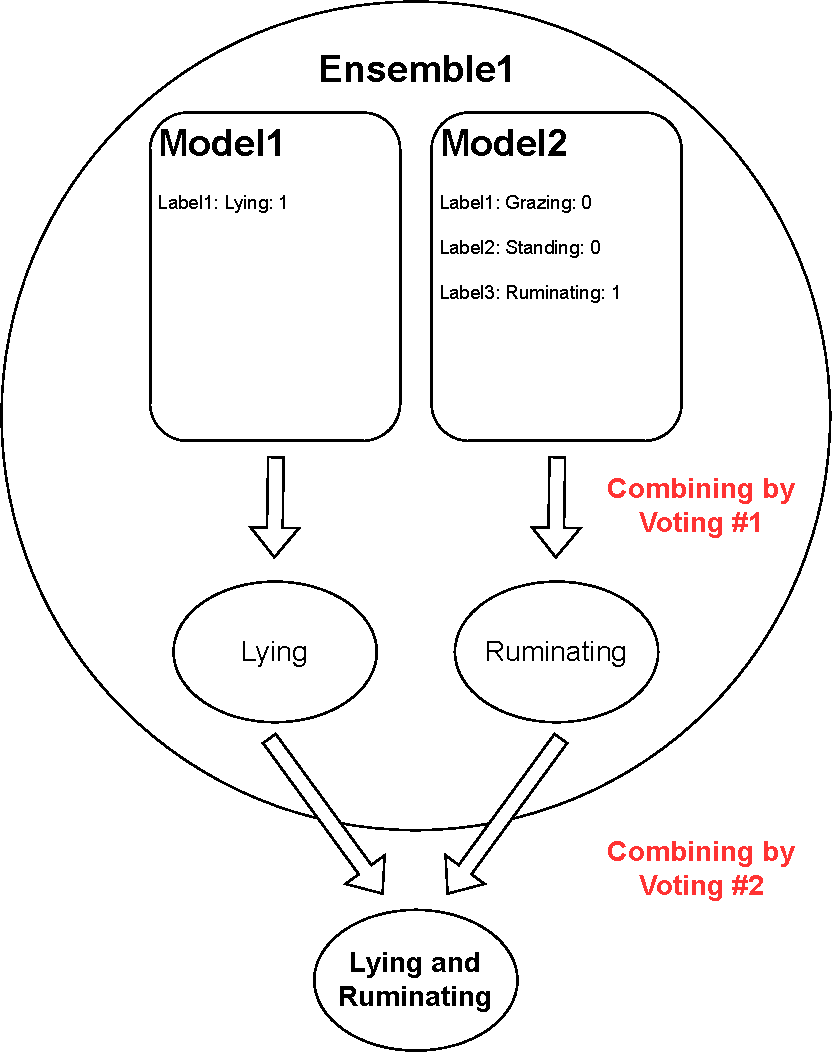
\includegraphics[height=9cm]{graphics/combining.pdf}
      \captionof{figure}{Combining the classifications into one final label}
      \label{fig:combining}
    \end{minipage}%
    \begin{minipage}{.5\textwidth}
      \centering
      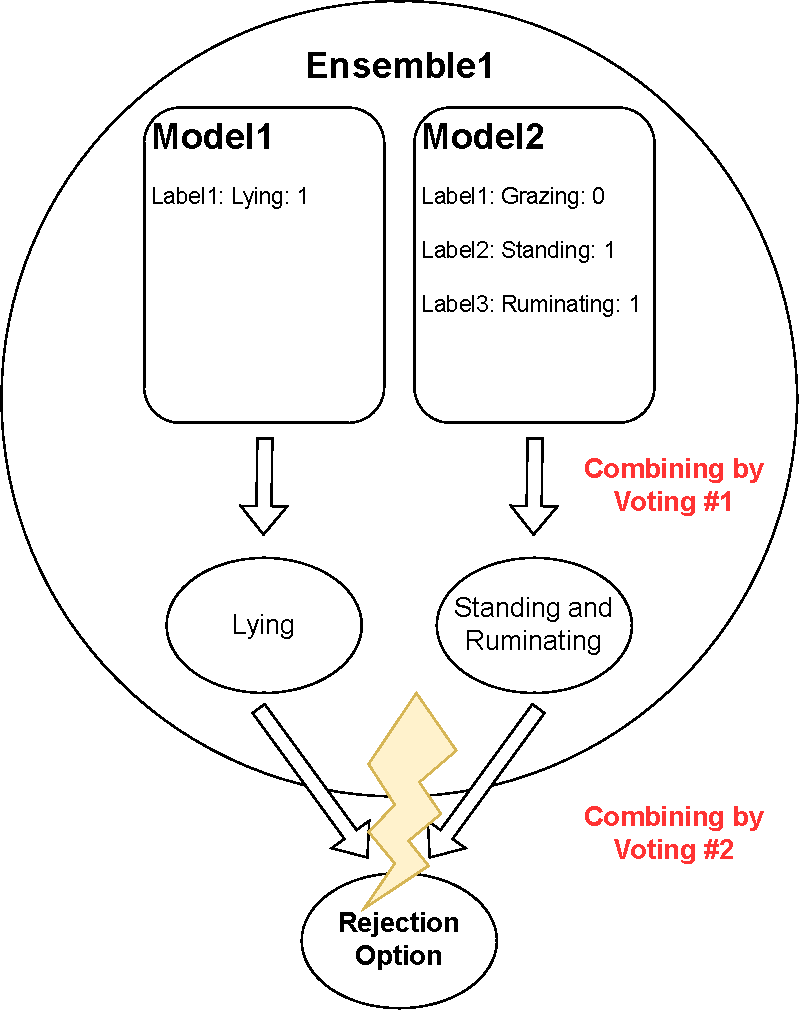
\includegraphics[height=9cm]{graphics/combiningrejection.pdf}
      \captionof{figure}{Rejection option, as lying and standing are exclusive behaviors}
      \label{fig:combiningrejection}
    \end{minipage}
    \end{figure}


Combining the predictions of each classifier brings some crucial benefits to the overall system that impact various aspects of the underlying use case. For one, having displayed only one final result will lead to a much more user-friendly interface. Domain experts or Data Scientists will not have to manually check the prediction of all components of the model set anymore but rather can see the current classification instantly, without having to consider the result of every model on its own. Especially when using larger model sets, the likeliness of errors made by manual human calculation will drop to a minimum. 

During the development stages for this work, it became evident that most ensembles, that were introduced in this section, are not an optimal solution for either use case. Even though some form of voting mechanism is essential for CAR in order to categorize any time interval into one category only, a classic ensemble method like Bagging or Boosting does not seem to be perfectly applicable to this use case. While Stacking seems to be possible for combining the votes for cattle behavior, it comes with expensive resource costs that would contradict the aim of creating a resource-aware system. It must also be noted that combining votes from individual models inside an ensemble is not the focus of this work. Instead, the focus will be on the model selection and retrieval process. Therefore, the outlined approaches regarding combining votes will not be addressed any further. 

Regarding the PAP, predictions from different single models don’t necessarily have to be combined, as they are interpretable and valid on their own. Therefore, a traditional ensemble method would not be relevant for this use case anyway. Instead, a looser combination of different models needed to be created. The implementation that will be introduced in \autoref{chap:implementation} is an attempt to create such combinations. Since the priorly introduced ensemble methods are not entirely practical for PAP and combining votes is not the focus of this work, the term model set will be used to refer to a combination of models from now on. Model sets therefore describe a combination of models whose results do not necessarily need to be combined. Nevertheless, the basic introduction to the topic of ensembles is valuable to gain a deeper understanding of the theoretical foundations of combining machine learning models. As mentioned above, the theoretical concepts, the design, and the implementation that were done for this work mostly refer to the PAP use case. However, the paradigm developed in the course of this work can also be applied to other use cases, in particular the CAR project. 


\section{Resource Awareness} \label{sec:ra}

The following section will give an overview of the topic of resource awareness, by describing it and discussing what metrics could be used to measure resource awareness. In machine learning, resource awareness is applied to various stages of the holistic life cycle of a model. Many previous works \cite{amir2018,tann2016,yu2018} focus on making the inference phase more resource-aware, i.e. reducing the time and computation power needed for the model to produce predictions. Nevertheless, there has since been an increase in making the training process of models more resource-aware as well \cite{rapp2022}.

Resource awareness forms one of the two main pillars this work is focusing on, next to performance. While the two concepts are not necessarily canceling each other out - resource-aware models can definitely be well-performing as well and vice versa - they certainly describe two completely different ideals. This tradeoff between having models that can accurately predict or classify a certain problem, but also making sure that the available resources like memory and computing power are used as efficiently as possible, can generally be solved in one of two ways. One option is to formulate a constrained optimization problem, by defining a limit for a certain measure. An example could be the maximum amount of features a model should use, or the smallest window size one wants to use for preprocessing. The second option is to create a multi-object optimization that aims for an optimal compromise of both relevant measures, i.e. between performance and resource awareness \cite{feurer2019}. As it will become apparent in the following chapters, this work mainly focuses on multi-object optimization by using different weights to level out resource awareness against performance. In addition, however, there will also be an option to use the model set retrieval system as a constrained optimization problem by only creating model sets that use the same feature set.

A central topic of this work was the different stages of measurement of resource awareness. Sünkel et. al. assessed resource awareness using Query Sharing Levels (QSLs) \cite{sunkel2022}. In total, 5 different levels were defined, that describe the extent of properties two or more models share with each other. Each subsequent level is only achievable if the conditions for the previous level are reached. In the mentioned paper, level 0 describes a set of models that have no common qualities. Level 1 is reached, if the models share the same sensor system. If, in addition, the models have undergone the same preprocessing they reach level 2. The third level is reached if the models share the same segmentation (window size), and the highest possible sharing - level 4 - is only reached if the models also have the same features between them. As \autoref{chap:design} will show, the QSLs as proposed in \cite{sunkel2022} have been adjusted for this work. However, the general idea of using different levels to assess the extent of resource awareness between two or more models has been maintained.

By definition, QSLs can only be defined using two or more models. They are not a valid method to evaluate resource awareness on only a single model. This proves to be a rather problematic matter for the case of model set retrieval systems: Only at a late stage in the model set retrieval process, can resource awareness really be considered. A number of model sets have to be created first, in order to look at the extent of resource utilization of those model sets. This means that the learners that make up model sets would either have to be priorly selected based on their performance only (which would result in creating performance-heavy model sets only - the amount of resource-aware model sets could be really low as a result), or every single available model would be used for model set creation (resulting in a very resource costly operation in itself - the vast majority of the created model sets would never be considered in the retrieval process anyway). This problem of having only an option to address resource awareness for model sets and not for single models led to the development of two concepts called inter-model resource awareness and intra-model resource awareness. The extent of efficient resource utilization of a model set is then assessed by looking at that model set from two different perspectives. The main motivation for the development of inter-model and intra-model resource awareness as well as the options that were examined when designing the architecture of the model set retrieval system concerning resource awareness will be provided in \autoref{sec:designretrieval}.


\section{Performance} \label{performance}

The second pillar of this work, next to resource awareness is performance. As performance is a rather broad term and many different metrics can be used to measure the performance of a machine learning model \cite{erickson2021}, some clarification and delimitation of the term has to be made. Generalization performance is a term, that refers to a model's ability to correctly predict new data. It is a crucial point in assessing the quality of a learner and therefore greatly affects the model selection process \cite{hastie2009}. For simplicity, this work will use the term performance when referring to generalization performance. One way to categorize performance metrics is to divide them into four classes which will be introduced shortly: Accuracy-based metrics measure the accuracy of the predicted result in comparison to the true result. Examples of accuracy-based metrics are accuracy in percent, F1, precision, and recall. Error-based metrics on the other hand determine the performance of a model based on the error in prediction between the predicted and the actual value. Mean Absolute Error (MAE), Mean Squared Error (MSE), and Root Mean Squared Error (RMSE) are examples of error-based metrics. Investment-based metrics are of relevance when working with algorithms whose purpose is to come up with investment strategies and usually give context about the risk and reward of a specific strategic approach. Finally, all other informative metrics can be summarized into a miscellaneous category. The metrics of this class usually provide supplementary information that enhances the previously introduced classes of performance metrics \cite{dessain2022}. This work will focus on error- and accuracy-based metrics, namely on accuracy, MAE, MSE, and RMSE.

The idea of using accuracy as a metric of performance seems straightforward, which may be a reason for its popularity in evaluating a machine learning model in the first place. Accuracy provides a general measure of how correctly the model is predicting across the entire dataset. It specifies, with what probability a new data point is predicted correctly \cite{grandini2020}. While this seems very unambiguous for classification problems (either a model predicts the correct behavior of cattle or it doesn’t), there are various things to consider when working in a linear regression setting. If a model would have to predict the occupancy for a parking lot with exact precision (including potential decimal places), probably not many models would have an accuracy value that is considered acceptable. One approach to fix this could be to add a tolerance value when calculating the accuracy of a classifier. If the prediction falls into an interval of $[v-t, v+t]$, where $v$ is the true value and $t$ is the tolerance value, the prediction will be classified as correct. As \autoref{chap:implementation} will show, this approach is applied in this work using the metric \texttt{accuracypercent}. However, the solution that is usually applied for linear regression problems refers to an error-based metric instead, mainly MSE. This way, it can be measured how closely the predicted response value matches the true value for an observation \cite{james2023}. MSE uses a dynamic to have a bigger deviation from the true value increase the error metric exponentially more than smaller deviations. As with all other error-based metrics, a lower score indicates a better-performing model. MSE is calculated using

\begin{equation}
\operatorname{MSE} = \frac{1}{n} \sum_{i=1}^n(y_i - \hat{f}(x_i))^2,
\label{mse}
\end{equation}

where $y_i$ is the true value, and $\hat{f}(x_i)$ is the predicted value.

A similar error-based metric that is widely used for assessing the performance of a model is MAE, which removes the additional penalty for larger deviations from the true value, by averaging the net deviation from the true value without squaring it. It is assessed using 

\begin{equation}
\operatorname{MAE}(y,\hat{y}) = \frac{1}{n} \sum_{i=1}^n |y_i - \hat{y}_i|.
\label{mae}
\end{equation}

Finally, RMSE is used to bring the values of MSE into a usable dimension by taking the square root of MSE. Because of this, the metric is in the same unit as the independent variable, i.e. between 0 and 1 for PAP. Consequently, RMSE is calculated using
\begin{equation}
\operatorname{RMSE} = \sqrt{\frac{1}{n} \sum_{i=1}^n e_t^2 }.
\label{rmse}
\end{equation}


Having defined what performance means in the context of machine learning models, as well as having introduced the metrics for assessing performance in this work, a basic understanding of the two pillars of this project - performance and resource awareness - has been conveyed. 



\section{Top-K Retrieval}\label{sec:topk}

The overall idea of top-k retrieval is straightforward: The user determines a number $k$ of objects they want to receive, and the retrieval algorithm returns the $k$ best items back to the user. As there are numerous variables, settings, and underlying algorithms to consider when using top-k retrieval, the following section will give a brief overview of the topic. 

Before items in a dataset can be assessed for ranking, it must be determined according to what metric(s) those items should be ranked. This is done by using a so-called ranking function, that describes the criteria for the items score that is later used for the actual ranking and selecting of items. A simple ranking function for instance could be the accuracy of a machine learning model. Each model (i.e. item) in the dataset has an assigned accuracy metric in addition to its unique identifier (i.e. primary key). A trivial ranking function could now rank these models according to their accuracy in an ascending or descending order. However, this gets continuously more complicated the more attributes are added to the ranking function: For instance, let us assume that there is another attribute for each machine learning model in the dataset that describes the number of features that were used to train that model. A possible ranking function could now consider both metrics, assigning the model a higher score the higher the accuracy and the lower the number of used features. The general method of ranking the items now is to assess both relevant metrics of an item, apply the ranking function by calculating a score using the (normalized) metrics and optional weights, and ranking every assessed item using this newly computed score. 

A naïve algorithm (NA) would now do this to every item in the database and then output the $k$ items with the highest scores. It is obvious, that such an approach would lead to long retrieval times and computational costs as it would need to consider every single item in the table – even those, that are not nearly close to the top $k$ items. As the costs for this algorithm are linear to the number of total items, it would not be an efficient form of retrieval for databases containing a large number of items \cite{fagin2002}.

Numerous algorithms have been developed in the last decades to utilize a more cost- and time-effective method for top-k retrieval, two of which will be introduced in the following subchapters. A mutuality of those algorithms that is worth examining before going into more detail about their characteristics is the way the data entries are handled: Before the actual calculation of scores can happen, the algorithms first split the database into smaller lists, each containing only two attributes: the relevant attribute that is to be considered for calculation of the score of an item (i.e. performance or resource awareness) and its respective primary key. Therefore, in the example stated above the database would now consist of two lists, one containing the primary key and the accuracy of each model, and the other containing also the primary key in addition to the number of features used to train said model. These lists are then sorted in descending order of the relevant metrics value (and not the primary keys). Consequently, each value gets assigned a grade, depending on its position in the sorted list. The item that has the topmost position in a list therefore has the best grade.

When describing top-k techniques, two types of data access are generally considered that are crucial to understand. The first one is called sorted access and defines obtaining a metric of an object by advancing through the corresponding list sequentially until the according value is reached. Therefore, to access a metric, or score of an item that has the $l^{th}$ best grade in a list, $l$ sorted accesses have to be made in order to obtain this value. NA does $n$ sorted accesses at all times, where $n$ is the number of objects in a list. The other mode of access is called random access. In contrast to sorted access, here the grade of a certain object is identified directly in one step. Instead of having to increment through any other items, the desired grade is accessed immediately. As a drawback, however, random access is often expensive or not even possible in certain scenarios.

With the clarification of these definitions, FA and TA can now be properly introduced.



\subsection{Fagin's Algorithm}

As the name suggests, FA was first introduced by Robert Fagin in 1999 \cite{fagin1999}. Provided that the dataset is already split into separated lists as stated above, an appropriate number $k$ and a scoring function is chosen, the algorithm works as follows:

\begin{enumerate}

\item Sorted access is done to each sorted list in parallel, meaning that first the best-graded metric in each list is accessed, then the second-best metric, and so on. (It is important to understand, that by doing this, not necessarily all metrics of one single object are being accessed at the same time, as an object can have a high grade in one metric, but a rather low one in another metric – which would therefore only be seen after a certain number of sorted accesses in the corresponding list. This sorted access is done until $k$ objects have been seen completely in every list. That means all metrics of at least $k$ objects have been seen through sorted access. 

\item For each object $R$ that has been seen, but not completely seen (meaning at least one grade of $R$ has not been accessed yet), all missing grades from $R$ are accessed through random access. 

\item The overall score is calculated for each object that has been seen using the scoring function. The objects are then sorted by their overall score and finally, the $k$ objects with the highest score are returned. 

\end{enumerate}

It has been proven that under the circumstance of a strict scoring function, FA operates optimally. A scoring function is defined as strict if the overall score of an object reaches its maximum of $1$ when each metric of this object also reaches its maximum value of $1$. However, several situations can be identified, where a scoring function would not behave in a strict manner, for instance when the scoring function is a constant or depicts the maximum value of an object's metrics. In both cases, other algorithms would outperform FA \cite{fagin2002}. Because of such restrictions in the performance of FA, another approach for top-k retrieval shall now be introduced.


\subsection{Threshold Algorithm}

TA first appeared in 2002 after a number of other similar algorithms have been independently developed that aim to solve the same problem \cite{fagin2002a}. Its procedure is as follows:

\begin{enumerate}

\item Much the same as in FA, sorted access is done in parallel in each sorted list. However now, for each seen object $R$, the remaining metrics of $R$ are gathered directly through random access, and $R$'s overall score is calculated using the scoring function. $R$ is stored together with its overall score if it is one of the $k$ highest scores that have been seen yet, breaking ties arbitrarily. 

\item For each sorted access a threshold value is created that consists of calculating an overall score using the metrics that are obtained in this sorted access. In other words, the accessed grades are used to calculate an overall score of a hypothetical object that consists of these accessed grades.  The sorted access is stopped as soon as at least $k$ objects have been seen whose overall score is equal to or higher than the computed threshold value. 

\item The $k$ objects with the highest score that have been stored are returned.

\end{enumerate}
 

 The way the TA is designed, it always has less or equal sorted accesses as FA. In addition, as at most only the $k$ objects with best scores are stored at any time, the required buffer size is noticeably smaller than with FA. The buffer of the latter in contrast can grow quite large as FA remembers every seen object in sorted access \cite{fagin2002}.

% TODO Decide whether or not to include graphics of the algos


\subsection{Additional Top-K Approaches}

Numerous other algorithms have been developed that aim to retrieve the best $k$ items in accordance with a scoring function. Particularly worth mentioning here is the No Random Access algorithm, also developed by Fagin \cite{fagin2002a}. As the name suggests, this algorithm tries to minimize the number of random accesses made to the sorted lists. Overall, all of the top-k processing techniques that focus on the way data is accessed can be summarized into a larger group of top-k methods. However, apart from the way data is accessed, top-k approaches can also be categorized by their proximity to and integration into the underlying database engine \cite{ilyas2008}. Newer approaches, that are characterized by their close relation to the query engine, for instance, include rank-aware query operators or concepts like Group-Ranking \cite{li2006}. Another technique that shall not be unmentioned is the Skyline operator \cite{borzsony2001}. This approach is characterized by not using any form of a scoring function. Instead, multiple objects that dominate other objects in the relevant metrics are returned - similar to a skyline where buildings that are either taller or nearer to the viewer can be seen. It therefore follows that the topmost ranked object for each metric is automatically returned using the Skyline operator. 

While significantly more approaches to top-k retrieval exist \cite{ilyas2008}, the introduced algorithms in this section shall be sufficient for this work. Because of the sheer amount of available top-k methods, the following chapters will focus on the most straightforward and established ones: NA, FA, and TA. Choosing these data access-based top-k algorithms also has the advantage that the number of accesses can be seen as an indicator for resource awareness. This is why the amount of sorted and random accesses will be one of the evaluation metrics in \autoref{chap:evaluation}. Other methods for ranking objects like the Skyline operator contradict certain relevant points in the introduced use cases, like the idea of having a fixed scoring function. Assessing those miscellaneous top-k approaches therefore goes beyond the scope of this work and will not be further addressed. The advantages of FA and TA will be made apparent by comparing their execution time and the number of accesses to that of NA in \autoref{chap:evaluation}.
With the theoretical foundation having been laid out, the next chapters, however, will first be dedicated to the practical sides of the model retrieval process by introducing the development done for this work.
\chapter{Design and Architecture} \label{chap:design}

For a model set retrieval system to be working properly, of course, there need to be machine learning models to choose from in the first place. Therefore, next to the design and implementation of the actual top-k algorithms, a diverse and extensive model database first had to be established. This chapter on architecture and design, as well as the following chapter that focuses on implementation, will describe the development process of both a top-k retrieval system as well as a training pipeline that was established to automatically preprocess data and train machine learning models based on this data. To understand the relationships between the modules developed in this work along with the used databases, \autoref{fig:globalarch} gives an overview of the general model creation and retrieval process. The workflow usually starts by the user starting the preprocessing pipeline which produces the data that can later be used for training models. Next, the user specifies which models they want to automatically train and store and then runs the training pipeline. The created models are then saved in a model database. As a third step, the user might want to retrieve the best $k$ model sets out of all created models. They then specify the necessary settings in a client, which sends the corresponding request to the retrieval system. After obtaining the relevant models from the priorly filled model database, the retrieval system then creates model sets out of the best models and finally returns the $k$ best model sets back to the client, which displays them to the user.

\begin{figure}[htbp]

  \makebox[\textwidth][c]{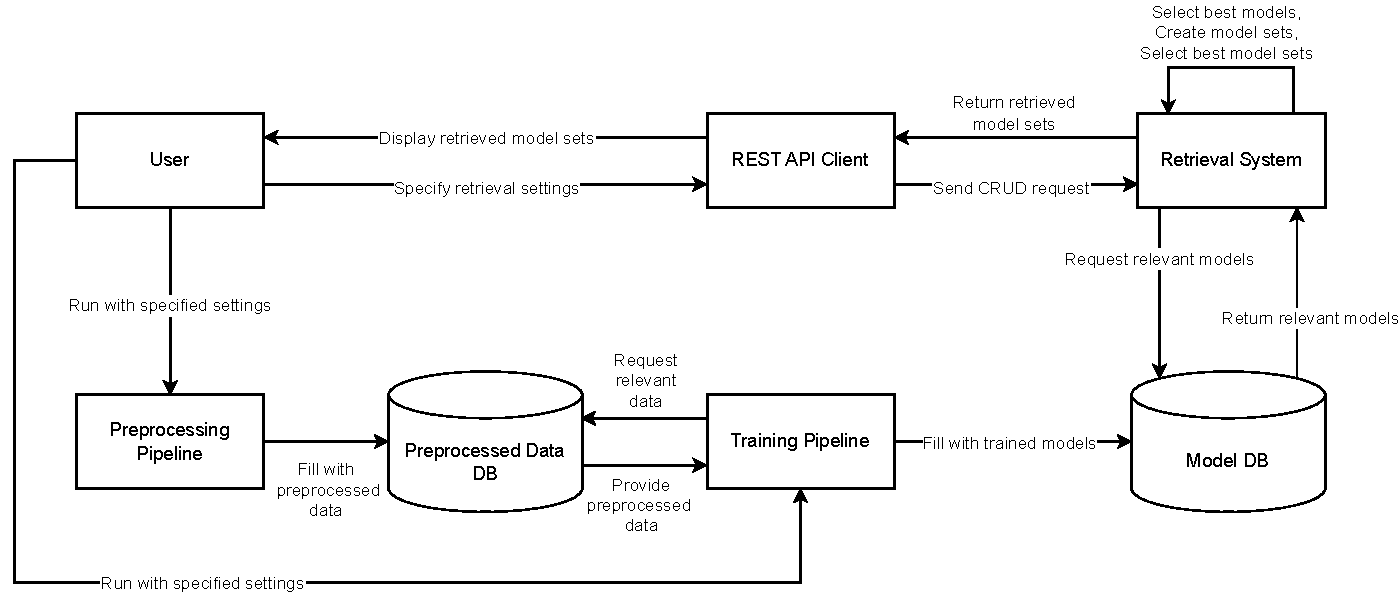
\includegraphics[width=1.1\textwidth]{graphics/globalarchitecture.pdf}}%
  \caption{The Architecture of the Different Modules and Databases in This Work}
  \label{fig:globalarch}
\end{figure}

\section{Training Pipeline}

%TODO Das hier in Implementierung schieben! 
The first section that was worked on when starting this project, is the training pipeline. First versions of a model trainer have already been developed by fellow students Paul Pongratz and Alexandr Litvin in previous semesters. This original form of a module that could train machine learning models for the use cases introduced in \autoref{chap:relatedwork} served as a valuable basis to improve upon. The model trainer was written in Java and used the Weka (Waikato Environment for Knowledge Analysis) \cite{eibe2016} library as its main building block. Weka is an open-source software that specializes in machine learning and data mining. With the help of this library, data entries of the parking behavior including time stamps and weather information can be converted into so-called \texttt{Instances} which are then used to train different kinds of classifiers such as Linear Regression or Random Forest which are also managed by Weka. In addition, the library was used to apply filters, in order to make use of different feature-scaling methods. To get the relevant parking data that is stored in a \texttt{postgres} database on the university's servers, a Java \texttt{DriverManager} of the library \texttt{java.sql} is used. That way a connection to the \texttt{postgres} database is established and a SQL statement with the relevant information is both created and executed. Another library that was essential in the creation of the model trainer is \texttt{tablesaw}, which makes it possible to create and manage data into \texttt{dataframes}, similar to the \texttt{pandas} library in Python. \texttt{Tablesaw} is mainly used to establish training- and testing-datasets out of the data queried from the database. Some exemplary usages include counting rows, dropping columns, or joining tables. Because the original model trainer was written in Java, and the development of the training pipeline was done using the model trainer as a template, a constraint for the training pipeline was that it should also be implemented using Java.

Regarding the overall architecture, the training pipeline initially was constructed in a way that let the user put in the desired model settings in a \texttt{config.properties} file which then was read by an \texttt{InputStream} to populate an object of the class Settings. This of course had to be modified in a way, that had the properties file be filled in automatically. Additionally, in the original version of the model trainer, the relevant data was pre-processed for each model, which turned out to be a very time-consuming effort. It was therefore decided to introduce a second entry point to the model trainer java program that takes care of all the pre-processing of the data entries. The pre-processed data is then stored in a separate database, which is later accessed by the actual model trainer for training and testing. The implementation chapter will go into more detail regarding the actual integration of those classes.

\section{Retrieval System}\label{sec:designretrieval}

The general aim of implementing the model set retrieval system was to provide the user with a highly customizable option to retrieve models and model sets that are tailored to their needs and the specific use case, whilst relying on different algorithms that have been well established in prior scientific work. This subchapter aims to give an overview of the functionalities of the retrieval system as well as the development process. As the retrieval system was designed entirely from scratch, much thought went into conceptualizing it to fit the use cases as much as possible. The development of new theoretical concepts led to many iterations in the development of the retrieval system. While \autoref{fig:flowchartretrieval} and  represent the retrieval process in final form, the following paragraphs will explain the design of the retrieval system more chronologically regarding the development. % TODO Checken

\begin{figure}[htbp]
  \centering
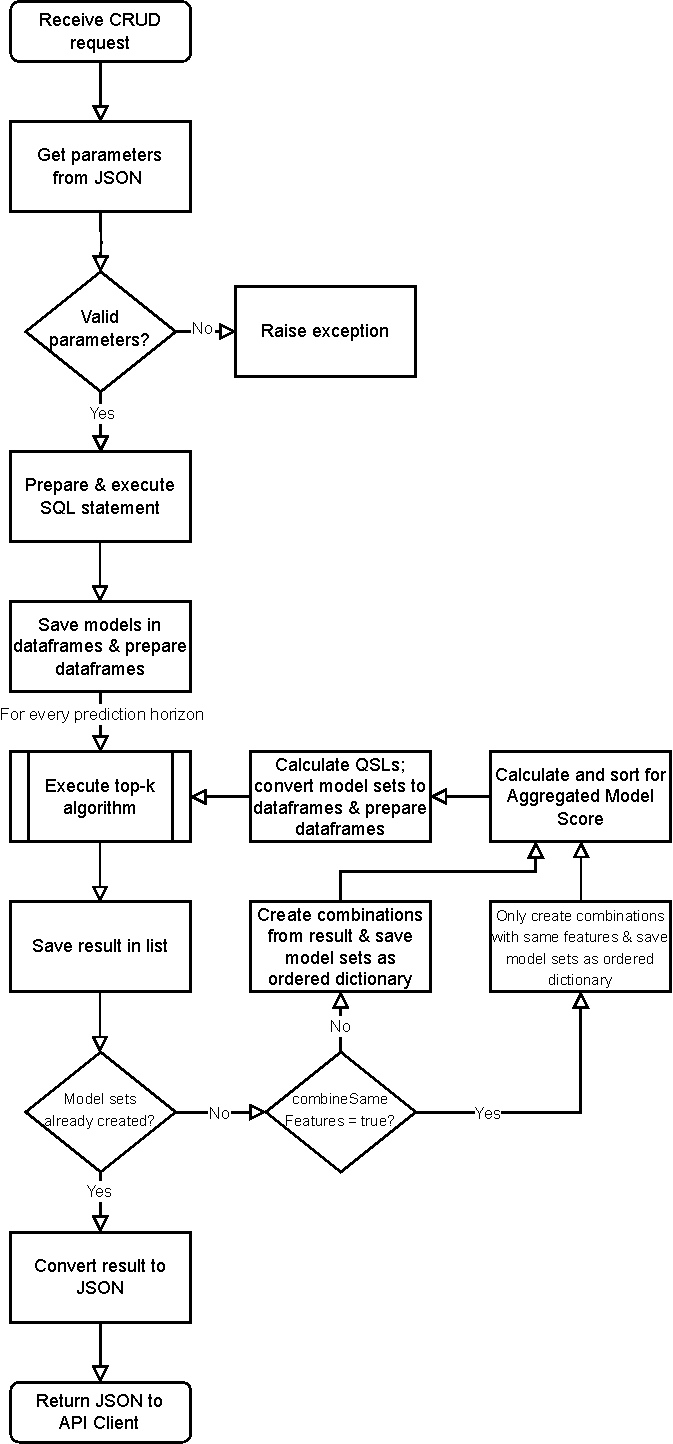
\includegraphics[height=14cm]{graphics/flowchartretrieval.pdf}
  \caption{Flowchart of the Top-K Retrieval System}
  \label{fig:flowchartretrieval}
\end{figure}

\subsection{Process of Retrieving Model Sets}

The procedure when retrieving the best model sets starts with the retrieval system receiving a call to an API endpoint. For that, the following endpoints have been established, the most important one for this work being the top-k retrieval for model sets.

\begin{itemize}

\item \textbf{Model selection} ( \texttt{/api/select}): CREATE operation that retrieves information about a model that the user specifies via a JSON file. 
\item \textbf{Model direct selection} (\texttt{/api/model/<model-name>}): READ operation, that retrieves information about a model the user specifies directly in the URL.
\item \textbf{Top-k single model} (\texttt{/api/topk}): CREATE operation that retrieves the $k$ best models based on the users' input.
\item \textbf{Top-k model set} (\texttt{/api/topk/modelsets}): CREATE operation that retrieves the $k$ best model sets based on the users' input.
\end{itemize}

\autoref{tab:settings} gives an overview of what settings the user can specify to customize their model set retrieval request. The description of the settings is followed by the possible values the settings can take on in the current implementation.


%  Retrieval System settings table
\begin{table}[htbp]
  \centering
      \begin{tabular}{  l  p{7cm}  p{3cm} }
          \toprule
  \textbf{Setting}      
  & \textbf{Description}   
  & \textbf{Values} \\\midrule
  
  pID & The parking lot ID that the model set should predict for & \texttt{38} or \texttt{634} \\\hline
  windowSize & The window size option(s) of the models inside the model set & \texttt{1}, \texttt{5} or both \\\hline
  perfMetric & The performance metric to be used to calculate the Performance Score & \texttt{acc}, \texttt{mae}, \texttt{mse}, \texttt{rmse} \\\hline
  k1 & Number of models to consider for model set creation per prediction horizon. E.g., if k1 = 3, for every prediction horizon the top 3 models will be chosen to then further create all possible combinations of model sets. When having two prediction horizons, this means $3 \cdot 3 = 9$ different model sets are created & \texttt{1} to \texttt{n}, where \texttt{n} is the maximum number of models found in the model database \\\hline
  k2 & Number of model sets to be returned to the user. Out of all created model sets in the first top-k round, the top $k2$ are then selected. Setting k2 to \texttt{max} will automatically return all created model sets. E.g., when having three different prediction horizons, \texttt{max} will return $3 \cdot 3 \cdot  3 = 27$ different model sets & \texttt{max} or \texttt{1} to \texttt{n}, where \texttt{n} is the maximum number of model sets that can be created using k1 models \\\hline
  predHor & The different prediction horizons to be considered in the model sets & \texttt{10}, \texttt{30}, \texttt{60} or a combination of those \\\hline
  perfWeight & The weight of the Performance Score in relation to the Resource Awareness Score. E.g. a value of 0.8 will compute the Model Score using 80\% of the Performance Score and 20\% of the Resource Awareness Score & Value between \texttt{0} and \texttt{1} \\\hline
  AMSWeight & The weight of the Aggregated Model Score in relation to the QSL Score. E.g. a value of 0.8 will compute the Model Set Score using 80\% of the Aggregated Model Score and 20\% of the QSL Score & Value between \texttt{0} and \texttt{1} \\\hline
  algorithm & The top-k algorithm to assess the top $k$ items for both rounds & \texttt{naive}, \texttt{fagin} or \texttt{threshold} \\\hline
  combineSameFeatures & Option that makes it possible to only create model sets where all models use the same features & \texttt{true} or \texttt{false} \\\hline
  calculateQSL & Aggregation function for determining the overall QSL of a model set & \texttt{min}, \texttt{max} or \texttt{avg} \\
          \bottomrule
      \end{tabular}
  \caption{Settings in the Retrieval System} \label{tab:settings}
  \end{table}
  
After receiving a request, the retrieval system is then to get the necessary parameters shown in \autoref{tab:settings} from the request, and to check whether the provided parameters are valid. If that is not the case, an exception is thrown with specific information telling the user how to adjust the parameters for them to be processed further by the retrieval system. Otherwise, the parameters are used to prepare a statement to retrieve the corresponding models from the model database. After that statement is executed and models related to the user's settings have been obtained from the database, they are saved in different groups according to their prediction horizon (which will be presented more elaborately \autoref{chap:implementation}) and prepared for the following steps. This preparation includes assessing and normalizing the performance metric and counting the number of features of each model (for assessing intra-model resource awareness, which will be discussed in detail in \autoref{sec:motivationRA} and \autoref{sec:defRA}) as well as putting all models in two lists each, one dedicated to performance, the other one dedicated to resource awareness. As explained in \autoref{sec:topk}, by putting the models into two lists, each containing one relevant attribute that is then considered for score calculation (i.e. performance and resource awareness), the actual top-k retrieval can be started. According to the user's preference, either NA, FA, or TA is executed for every group of models per prediction horizon.

Having completed the execution of the top-k algorithm as described in \autoref{sec:topk}, the $k$ best models are stored inside a list. If in the settings the user did not activate \texttt{combineSameFeatures},  every combination from one model of each prediction horizon is created, subsequently producing model sets out of the best $k$ best models. If \texttt{combineSameFeatures} is set to \texttt{true} however, combinations are only created if every model shares the same features, which will result in fewer model sets created. Next, the newly created model sets are prepared for the second top-k retrieval, which finally aims to retrieve the $k2$ best model sets out of all created sets. Therefore, the so-called Aggregated Model Score is calculated (which will be further introduced in \autoref{sec:scores}) using the single model values in each model set. The Aggregated Model Score will be the first attribute to be used for the second top-k retrieval round. The second attribute will be the QSLs, which are calculated and assessed according to the user's setting in \texttt{calculateQSL} in the next step of the retrieval pipeline. The model sets then undergo the same preparation steps as before: The two relevant attributes are normalized and the models are placed into two lists, one representing the Aggregated Model Score, the other one representing the QSL Score. It is noteworthy, that \autoref{sec:scores} will introduce each score in detail. The next step in the system is the second top-k retrieval, which uses the same algorithm as the first round and the \texttt{AMSWeight} specified by the user. Lastly, the resulting list of the $k2$ best model sets is converted to be properly returned and displayed to the user.

As the model set retrieval system focuses on the logic of retrieving the best model sets customized to the users' preferences manifested in numerous settings that have been made prior to the request, the design and implementation of a front end e.g. in the sense of a web app has been dispensed with. Whilst an easy-to-understand user interface that guides the user through the various functions of the model set retrieval system might lead to a more intuitive and time-saving engagement between the user and the system, this part was not the focus of this work and might be better suited for future development.



\subsection{Motivation of Restructuring Resource Awareness}\label{sec:motivationRA}

%  Das ist eine sehr gute Contribution in deiner Arbeit! Für den Leser wäre es evtl. gut, die Motivation dafür noch genauer herauszuarbeiten. Dem Leser ist die Abfolge der Schritte beim Retrieval ggf. noch nicht bewusst. Du schreibst hier von dem Schritt der "Model Set Creation". Warum ist es wichtig davor bereits intra-model resource awareness zu betrachten?
% Sollte der Leser an dieser Stelle bereits über die Retrieval-Pipeline im Bilde sein? evtl. solltest du diese Diskussion in ein späteres Kapitel verschieben? Und hier nur Einführende Statements schreiben? (Also Related Work zu Resource-Awareness und hier nur kurz andiskutieren, die Contribution lieber in einem späteren Kapitel und verlinken)

%TODO Folgenden paragraph durchchecken
The use case of selecting not only single items (i.e. single models) through a top-k retrieval system but rather composing whole sets of those items made it necessary to approach the design of this module with numerous extra steps in mind. Each model set should contain models of different prediction horizons, a metric that will be introduced in detail in \autoref{chap:implementation}. It is assumed that each model set contains either two or three different prediction horizons, and therefore two or three different models. The central challenge was to find a way to determine the resource awareness of a model set before actually composing that model set, which ultimately led to the introduction of intra-model resource awareness. The following paragraphs will be dedicated to showing the motivation behind inter-model and intra-model resource awareness. 

In a simple top-k retrieval system, items containing different metrics are sorted for each of those metrics. The items that should be returned in this use case are the model sets, whilst the relevant metrics are the performance (i.e. accuracy or an error metric like MAE) and resource awareness. This resource awareness however has been previously defined to be measured by ascertaining the underlying QSLs in that model set. As mentioned in \autoref{chap:relatedwork}, a straightforward approach would then have been to simply create model sets before retrieving them using a top-k algorithm. The accuracy metric could then be asserted by taking the average value of the models' accuracy values that are contained in the model set, for instance. The resource awareness metric could be easily measured by looking at the shared features of the models in the model set. The problem with this straightforward approach is, that a vast number of model sets would have to be created for it to work properly. Taking into account all the different metrics that a single model can have (e.g. window size, classifier, combination of features, …), all possible combinations of two or three of those models is a huge number to create. The database containing all possible model sets would have to be iterated through by the top-k algorithms, making the retrieval process slower than using a smaller database. Additionally, new model sets would have to be created every time new models are added to the model database, making it complex to manage and keep the model set database updated. 

Because of these reasons stated above, it was decided against using such a predefined model set database. A number of alternative approaches were designed at this point of the project, all approaching the resource awareness issues in different ways. They will shortly be introduced in the following section. 

\paragraph*{Alternative 1}
This approach is defined by neglecting the idea of having QSLs altogether. Instead, the resource awareness of a model set is supposed to be determined by establishing metrics of single models that represent the resource awareness. At this stage in development, the idea of having intra-model resource awareness assessed first came up. The metrics that were identified for this purpose were the number of features or the window size of a model. Using a top-k algorithm, the best models regarding both performance and resource awareness would then be searched and put into model sets. Depending on which prediction horizon is still missing in a model set, the best-rated model of both performance and resource awareness is then added to the set. 

\paragraph{Alternative 2}
Another possibility would be to calculate the QSLs at the end of the model set creation process. This approach starts the same way as Alternative 1, by finding the best models regarding performance and resource awareness using suitable metrics for either dimension as discussed before (e.g. accuracy and number of features). The single model retrieval would then continue until a model of each prediction horizon is found. (Or $k$ models have been retrieved, with each prediction horizon being selected at least once.) Subsequently, these retrieved models would be combined into every model set possible but under the condition that each model set includes the necessary prediction horizons. Ultimately the QSLs would be calculated and the model sets would be sorted according to their levels.

\paragraph{Alternative 3}
This approach is a modification of Alternative 2. It starts by creating lists of all models according to their prediction horizon. For instance, if model sets with three different prediction horizons should be created, three different lists would first be created. Thereafter, the $k$ best models for each prediction horizon would be retrieved and combined into all possible combinations. Ultimately the QSLs would be calculated and the model sets would be sorted according to their levels, just like in Alternative 2. The major difference between Alternative 3 and 2 is the number of models that are considered for model set creation. While in Alternative 2 only a few or maybe only one model could be considered for a certain prediction horizon, the number of models considered per prediction horizon is always the same in Alternative 3. 

\paragraph{Alternative 4}
This is the option that was ultimately decided to be used in the final implementation of the model set retrieval system. The main idea behind Alternative 4 is to combine the advantages of each of the previously introduced alternatives in order to create a retrieval design that works best for the required use case. For this, intra-model resource awareness metrics and QSLs are both used. First, the model database is split up into lists of each prediction horizon. Then, the $k$ best models for each prediction horizon are retrieved based on a constructed Model Score which is a combination of the models' performance and its intra-model resource awareness metric, using a top-k algorithm. Subsequently, the retrieved models are put into model sets by using every possible combination (whilst also respecting the condition to use a specific prediction horizon only once inside a model set). Another score called Aggregated Model Score is then created, which depicts the summarized Model Scores inside a model set. Afterward, the QSLs for each created model set are calculated. As a final step, a second top-k retrieval is started, in order to acquire the $k$ best model sets based on an overall Model Set Score that is created by weighting both the previously calculated Aggregated Model Score and the QSLs which act as an inter-model resource awareness metric. For this second top-k retrieval, a separate \texttt{k} and weight can be chosen in comparison to the first top-k algorithm, to fine-tune the request if necessary. The $k$ best model sets are then returned to the user, together with all their associated meta information and scores. In summary, the implemented model set retrieval system makes use of running two different types of objects through the top-k algorithms: First, the single models that are later to fill the sets with, and the complete model sets second. The user however does not have to undergo any additional steps in order to obtain the top $k$ model sets besides providing the desired settings - the model set retrieval system manages calling the different algorithm rounds on its own.


\subsection{Definition of Intra-Model and Inter-Model Resource Awareness}\label{sec:defRA}

As mentioned in \autoref{sec:motivationRA} and \autoref{sec:ra}, measuring resource awareness turned out to be a crucial subject in this work. This subsection will clarify the final definition of resource awareness in the context of this work. By minding the flowchart in \autoref{fig:flowchartretrieval} and the general process pipeline for the retrieval system it becomes apparent that the QSLs are only assessed at a late stage in the retrieval process. Up until that point, the focus would only be on selecting models that perform well. Trying to prevent the problems stated in \autoref{sec:ra}, namely having to create model sets out of well-performing models only (leading to performance-heavy model sets only), or out of every single model (resource-costly model set creation), led to the decision to create a way to assess it before model set creation, and therefore distinguishing between two different types of resource awareness: Inter-model resource awareness and intra-model resource awareness, two terms that have been formed for this work. While inter-model resource awareness refers to the extent of resource awareness inside a model set, for example by using QSLs as introduced before, intra-model resource awareness describes the amount of efficient resource utilization inside a single model. To do this, many different metrics can be considered. First and foremost, the feature set of a model tells a lot about the required resources when using said model in a prediction use case: The more features a model was trained on, the more data has to be transmitted to that model in production, making the required data transmission more extensive. As an example, two models A and B shall be considered. While Model A was trained based on the day of the week, month, current temperature and humidity, time slot in a day, and the occupancy value of the previous time slot, Model B's predictions only rely on the time slot in a day. While it might be safe to assume that utilizing a lot more data should make Model A's predictions more precise, it becomes also apparent that this utilization of available information does not come without a cost. While Model B only needs a simple integer value as input before it can return its prediction value, Model A needs an entire array of data points that first have to be gathered. In a production setting, especially accessing current weather information like temperature and humidity might be resource-costly and error-prone, making Model A much less resource-aware than Model B. 

The second intra-model resource awareness metric that was identified in the current work is the window size of a specific model. The higher resource costs for models with a small window size become apparent in the CAR use case: When a model works on little window sizes, data from the sensors has to be transmitted more often than when working with larger window sizes. The amount of transmitted data will sum up to a large total, once the prediction is done for a longer period of time, making a small window size a factor for high resource usage. In \autoref{chap:evaluation} it is assumed that the window size of a model in the PAP does not only refer to its segmentation in preprocessing but also to the frequency of its executions. A window size of 10 minutes, for example, means the predictor is run every 10 minutes. Following this premise, it becomes evident that even in this use case, a small window size makes a model less resource-aware, than a model with larger window sizes. 

In summary, by combining intra- and inter-model resource awareness, both performance and the efficiency of resource usage can be considered in an equal fashion during the entire model set retrieval process. In the stage of selecting suiting models for the model set creation, the extent of efficient resource utilization is already quantified through intra-model resource awareness, which makes it possible to only create model sets that precisely represent the user's request in regards to both performance and resource awareness. Inter-model resource awareness makes it further possible to gain additional insights into the resource effectiveness of a model set, by not only having to look at the models and their building blocks like window size or feature set but also at the relationship between the models.

\subsection{Query Sharing Levels}

The design of the QSLs has been generally adapted from Sünkel et. al. \cite{sunkel2022}. However, Level 1 and Level 2 have been disregarded in this work, as they describe aspects of alignments that are always automatically fulfilled in the context of parking prediction: Level 1 of the original QSLs is reached when two models use the same sensor system, while Level 2 is reached if two models have the same preprocessing. As all models were being trained on the same parking data that was gathered using the same sensor system, the relationship between all models is at least reaching Level 1.

Furthermore, while general preprocessing is in fact happening in the developed system for this work, it is vastly different from the preprocessing in the CAR use case: There is no sensor data that has to be combined in a way to get a certain metric, like with the accelerometer signal. It can therefore be argued, that because there is no preprocessing happening in PAP, all models have undergone the same preprocessing step: no preprocessing. Following this argumentation, all models predicting parking availability reach QSL 2. To create a bigger divergence in the QSLs and to further additionally reward model sets that share the same window size or feature set, it was decided against using the levels $2$, $3$, and $4$. Instead, if two models in the PAP use case do not share the same window size, their QSL will be $0$, even though they technically share the same sensor system and the same preprocessing. Consequently, the possible QSLs in this work are $0$, $3$, and $4$.

By designing the model set retrieval system in a way, that makes it possible to choose the aggregation function for determining the overall QSL of a model set, the user is given even more freedom in customizing the query. Note, that this is only relevant for model sets containing at least three models, as a set containing only 2 models does only have one QSL to be determined. Model sets with three models, however, make it necessary to compare three different pairs of models with each other. \autoref{fig:qsls} displays this behavior of QSLs inside a model set. 

\begin{figure}[htbp]
  \centering
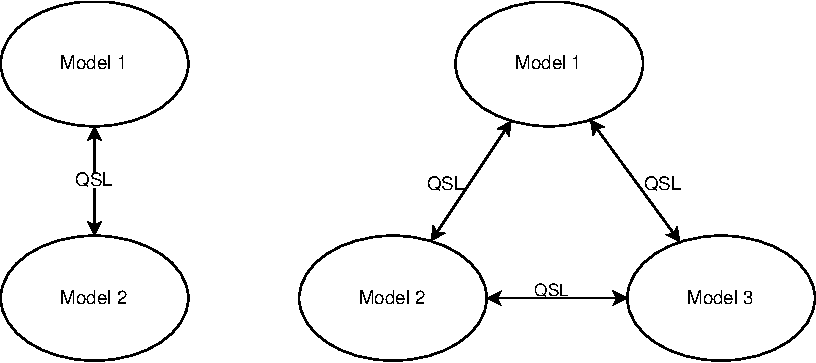
\includegraphics[height=4cm]{graphics/qsl}
  \caption{The Increasing Amount of Different QSLs in Larger Model Sets}
  \label{fig:qsls}
\end{figure}

Combining these individual levels therefore needs to follow an aggregation rule. For this reason, the possible options for calculating the QSL of a model set that have been designed are \texttt{min}, \texttt{max}, and \texttt{avg}. While with \texttt{min} the lowest level is chosen as the overall QSL for a model set, \texttt{max} chooses the highest level. \texttt{Avg} produces the mean value of all three measured levels.

A necessary addition to the QSLs was some form of normalization. As the value of the QSL of a model set will be combined with the Aggregated Model Score, both values have to be in the same interval in order to produce a meaningful Model Set Score that can be easily interpreted. It was therefore decided to introduce a QSL Score which is derived directly from the actual QSL. 
To transform the QSL into the QSL Score, \autoref{qslscore} is used, which was derived and modified from Sünkel et. al. \cite{sunkel2022}. Essentially, the formula puts the QSL Score inside an interval between 0.6 (if the QSL is 0 - no query sharing is possible) and 1 (if the QSL is 4 – same window size and features). This interval was chosen to fit the overall values that are to be expected in the Aggregated Model Score. 

\subsection{Scores}\label{sec:scores}

The following summary is intended to give a better understanding of all the metrics and scores invented and used for the model set retrieval process. \autoref{scoreconstruction} then shows how all those different scores are constructed and their relations to one another.

\begin{itemize}
	\item \textbf{Performance Score (PS)}: Score for a single model. Chosen performance metric (e.g. accuracy, RMSE,…) is normalized over all models retrieved from the model database in a query. Assumes a value between 0 and 1. Let $p_\text{min}$ be the minimum value and $p_\text{max}$ the maximum value of the performance metric across all models per prediction horizon, and let $p_\text{i}$ be the value of the performance metric of the model $i$, then
	\begin{equation}
    \operatorname{PS_i} = \frac{p_\text{i} - p_{\text{min}}}{p_{\text{max}} - p_{\text{min}}}.
    \label{ps}
    \end{equation}

  Note, that if error metrics are used for the calculation of the Performance Score instead of the accuracy, the Performance Score has to be reversed, so that low error metrics result in a higher score:
  \begin{equation}
    \operatorname{PS_j} = 1- \frac{p_\text{j} - p_{\text{min}}}{p_{\text{max}} - p_{\text{min}}}.
    \label{psrev}
    \end{equation}

\item \textbf{Resource Awareness Score (RAS)}: Score for a single model. The chosen resource awareness metric is normalized over all models retrieved from the model database. In the implemented version, this is a count of the used features of a model, with an additional penalty for small window sizes. The more features a model uses, the lower this score will be. Assumes a value between 0 and 1. Let $f_\text{min}$ be the minimum number and $f_\text{max}$ the maximum number of the features used across all models per prediction horizon, and let $f_\text{i}$ be the number of features model $i$ uses. Furthermore, let $pen_\text{ws}$ be the penalty that is added to the fraction if the observed model uses a window size of 1 minute. In the implemented version, $pen_\text{ws}$ is $3$.
\begin{equation}
  \operatorname{RAS_i} = 1- (\frac{f_\text{i} - f_{\text{min}}}{f_{\text{max}} - f_{\text{min}}} + pen_\text{ws}).
  \label{ras}
  \end{equation}

\item \textbf{Model Score (MS)}: Overall score for single model. Combines Performance Score and Resource Awareness Score using a predefined weight. 
\begin{equation}
 \operatorname{MS} = (\operatorname{PS} \cdot \operatorname{perfWeight}) + (\operatorname{RAS} \cdot (1- \operatorname{perfWeight})).
  \label{ms}
  \end{equation}

\item \textbf{Aggregated Model Score (AMS)}: Score for model set. Determined by calculating the mean value of the Model Scores inside a set. Let $n$ be the number of models inside a model set, then
\begin{equation}
  \operatorname{AMS} = \frac{\sum_{i=1}^{n} \operatorname{MS}}{n}.
  \label{ams}
  \end{equation}
  
\item \textbf{QSL}: Metric for model set. Depicts the degree of shared elements between two models inside a model set. Is determined for every 2-model combination inside a model set and subsequently ascertained for the entire model set by using one of three aggregation functions. Assumes value 0, 3, or 4 for each model-to-model relationship in a model set.

\item \textbf{QSL Score (QSLS)}: Score for model set. Derived from the QSL by using the normalization formula.
\begin{equation}
  \operatorname{QSLS} = \frac{(\operatorname{QSL} \cdot 10) + 60}{100}.
  \label{qsls}
  \end{equation}
  
\item \textbf{Model Set Score (MSS)}: Overall score for model set. Combines Aggregated Model Score and QSL Score using a predefined weight.
\begin{equation}
  \operatorname{MSS} = (\operatorname{AMS} \cdot \operatorname{AMSWeight}) + (\operatorname{QSLS} \cdot (1- \operatorname{AMSWeight})).
   \label{mss}
   \end{equation}
\end{itemize}


\begin{figure}[htb]
  \centering
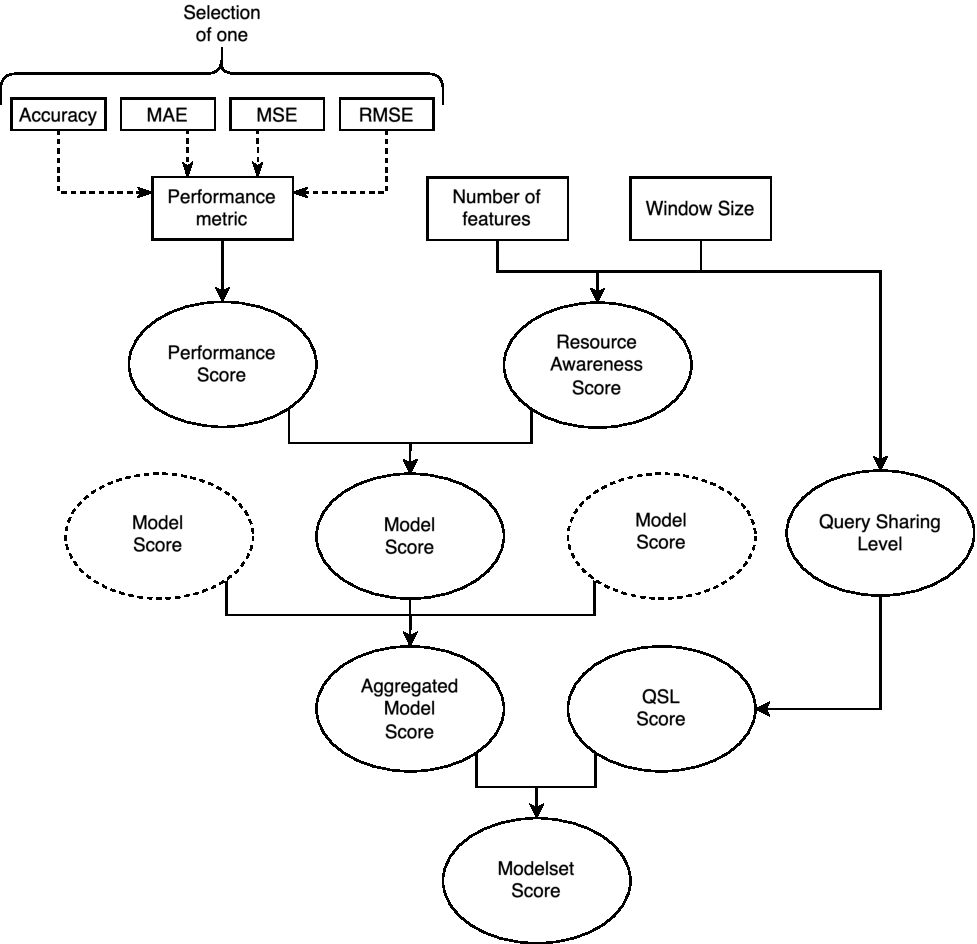
\includegraphics[height=12cm]{graphics/scores.pdf}
  \caption{Structure of the Different Scores Used for the Retrieval Process}
  \label{scoreconstruction}
\end{figure}




\chapter{Implementation}\label{chap:implementation}

The following chapter will give an overview of how both the latest version of the training pipeline as well as the model set retrieval system was implemented, how the user can customize the retrieval process by changing certain settings, and what challenges were faced during the implementation process.



\section{Model Database}

As mentioned in the previous chapter, there were many fundamental things to improve upon the already existing training-pipeline, when the development phase for this project was first started. The first step was to revise the model attributes by critically thinking about what information a machine learning model in the database should contain. As a result, the following attributes were added to the models in the database:

\begin{itemize}
	\item \texttt{model\char`_id}: Simple serial integer value that serves as primary key and makes it possible to refer to every created model in a precise way.

	\item \texttt{developer}: Attribute that makes it apparent, who trained and stored a specific model.
\item \texttt{created\char`_time}: Timestamp of when the model was successfully stored in the model database. 
\item \texttt{model\char`_size\char`_in\char`_bytes}: Integer value of the memory size of that specific model in bytes. This value is calculated by returning the length of a byte array that is filled using a ByteArrayOutputStream on the content of the classifier.
\item \texttt{training\char`_weeks}: Shows how many weeks’ worth of preprocessed training data was used to train a model. In the previous version of the training pipeline, one had to specify the amount of data entries (and therefore rows of raw parking data) that should be used for training. With the rework, the user now specifies the training data size in weeks instead. It is important to note, that for a fixed trainingWeeks value, a small window size value leads to more data entries used, than a big window size.
\item \texttt{window\char`_stride}: For the sake of completeness the window stride was added as a model attribute and depicts the time difference between the start points of two consecutive data entries used to train a model. In the present use case, the window stride is always the same as the window size.
\item \texttt{start\char`_of\char`_training\char`_data}: Depicts the month and year of the first entry of training data that was used for a model.
\item \texttt{prediction\char`_horizon}: The newly implemented prediction horizon of a model in minutes. Further information about this metric will follow in the next chapters.
\end{itemize}

In addition, the following attributes are reworked versions of previously implemented attributes. They were changed, either to be more comprehensible and uniform with the rest of the projects’ terminology or to refactor the actual values to be better tailored to the implementations’ functionalities.

\begin{itemize}

\item \texttt{model\char`_name}: Instead of choosing an arbitrary name for a model, the model\char`_name attribute was reworked to automatically give a model a standardized name based on its specifications, which makes it easy to extract important information without having to look up each metric separately. The syntax for the naming convention is as follows: \\\texttt{Classifier-Features-WindowSize-TrainingDataSize-ParkingLotID- \\PredictionHorizon-potentialSpecialProperty}. The features are separated by commas and are indexed as seen in \autoref{indexfeatures}.


% Indexing of features
\begin{table}[h]
\centering
    \begin{tabular}{ l | c}
        \toprule
\textbf{Features} &
\textbf{Index}      
 \\\midrule

temperature & 0 \\\hline
humidity & 1 \\\hline
weekday & 2  \\\hline
month & 3 \\\hline
year & 4 \\\hline
time\char`_slot & 5\\\hline
previous\char`_occupancy & 6 \\
        \bottomrule
    \end{tabular}
\caption{Indexes of the features used for training} \label{indexfeatures}
\end{table}


\item \texttt{training\char`_data\char`_size}: Previously called \texttt{table\char`_length}, this attribute states the total number of rows of preprocessed training data that were used for the training of this model. The value is calculated using the following formula: $training\char`_weeks \cdot 7 \cdot \frac{1440}{window\char`_size}$.
\item  \texttt{attributes}: Gives information about the attributes that were used to train this model. Instead of showing “all”, if every possible attribute was used in training, in the overworked version now every single attribute is listed for better readability. 
\item  \texttt{classifiers}:  The same improvements that were underdone for attributes were applied to the classifiers attribute for better readability. 
\item  \texttt{accuracy}, \texttt{mae}, \texttt{mse}, \texttt{rmse}: A models performance metrics. In the initial version of the training pipeline, these metrics were calculated and put into one single column, making it unwieldy to process further in the top-k algorithms (As an example, in previous versions of the top-k retrieval system, the accuracy values had to be extracted using a \texttt{re.search} function on the string that contained all the metrics, and then converted to a float value). By making the metrics atomic, they can be accessed more directly without wasting computational resources. Another advantage is the better readability for the user.
\item \texttt{space\char`_ids}: Previously called \texttt{slotids}.
Indicates which parking spaces were considered for training. In the executed pipeline-runs, every parking space was selected.
\item  \texttt{model\char`_content}: Byte array of the model. In the original training pipeline the content of the model was split into four different attributes, one per classifier. As there is only one classifier used per model, this was changed to always display the content in this attribute.
\end{itemize}

The following attributes were mostly adopted directly from the previous implementation, but will be introduced anyway to give context about their meaning:

\begin{itemize}
	\item \texttt{parking\char`_id}: The ID of the parking lot the model is trained on. In the current state, the parking lots 38 and 634 are available.
\item \texttt{window\char`_size}: The window size of the data entries used for training. This value describes how many minutes of parking activity should be summed up into one row of training data in the preprocessing phase. The models that were trained using a prediction horizon have a window size of 1 or 5.  
\item \texttt{trainingdataproportion}: Shows the proportion of the training data in relation to the test data. A value of 0.8 for example puts 80\% of the data into training, and 20\% into testing. 
\item \texttt{accuracypercent}: Metric that decides how many percent points the prediction of the model can deviate from the actual target value without being categorized as a wrong prediction. 
\item \texttt{randomforestmaxdepth}: Hyperparameter for Random Forest classifiers. The maximum number of splits each decision tree in the Random Forest can make.
\item \texttt{kneighbours}: Hyperparameter for KNN classifiers. The number of neighbors of a data point that should be checked for classification. 
\end{itemize}

The combination of these attributes made it straightforward to both filter for models when searching for something specific in the database, as well as process relevant information for the retrieval system.




\section{Training Pipeline}

With the structure of the model database explained more insight into the training pipeline can now be given. The functionality of the original model trainer was to create single models by specifying their properties in a \texttt{config.properties} file. After a new \texttt{Settings} object has been created that reads the \texttt{config.properties} file through an \texttt{InputStream}, a connection to the model database was established. Subsequently, the raw parking data was queried from the database and then preprocessed according to the specified properties. The preprocessed data was then used to build, test, and finally store the model in the model database. The process was then ended. It was apparent that simply implementing a repeating sequence of this process was not sufficient for a working training pipeline. Especially the recurring opening of new connections to the database was an obvious thing to be optimized. By restructuring the way the function \texttt{createDBConnection} is called, not only the problem of only establishing five connections at a time could be bypassed, but more prominently vast time savings could be accomplished. 

The general functionality of the training pipeline is based on several nested for-loops, each referring to one metric that is to be changed. Therefore, one for-loop is for example changing a predefined variable that stores the window size that should be iterated over. In order to make an insight into, as well as possible changes to the values in an uncomplicated manner, most of them have been stored in \texttt{HashMaps}. A \texttt{HashMap} may store additional information as well, and so the \texttt{windowSizeMap} also contains the values of \texttt{trainingWeeks} that are attached to the window sizes. In order to provide the model trainer with those changing properties of each new model that was to be built, a new function \texttt{changeValues} was implemented. Using a \texttt{FileOutputStream}, the values of the iteration are filled into the properties file, which was renamed to \texttt{training.properties}. During several test runs of the model trainer, however, it was noticeable that the changes to the properties file only came into force one iteration after the actual change. The reason for this was that changes in the \texttt{FileOutputStream} were only reloaded after each iteration. The \texttt{Settings} class therefore had to be modified in a way, so that it takes the already changed \texttt{Properties} object as an input parameter. The afterward created \texttt{ModelTrainer} object then directly refers to the changed values of the current iteration. 

A first longer test run led to the fixing of some minor problems, one being the handling of double-training the same models: The original model trainer was built in a way that encoded the features a model should be trained on by assigning each feature to a number. Deselecting all features, let to the training of all of them. Although, by selecting every number, the same result was achieved. Such unexpected behavior was adjusted by modifying the for-loops. More importantly, however, another inefficiency was addressed in this development stage. As the models mainly used the same subset of training and testing data, the \texttt{preprocessing} function was operating on the same data each time a new model was created. It was then decided to outsource the preprocessing phase into its own class \texttt{Preprocessor} and define a new database table that would store the preprocessed data for it to then be accessed directly by the model trainer as needed. Essentially, a second pipeline was therefore created that would take care of preprocessing data in reference to certain properties that have been set beforehand. The general procedure in this new preprocessing pipeline is very similar to the way the training pipeline works: The user uses the \texttt{HashMaps} to set up the parking lots and the window sizes that should be preprocessed on. A \texttt{changeValues} function that is similar to the one used in the \texttt{ModelTrainer}  then changes the values in a \texttt{preprocess.properties} file via an \texttt{FileOutputStream}. After that, the raw parking data is queried from the database and is then preprocessed by segmenting it into windows of the previously set size. The window size is the same as the window stride, leading to sliding, non-overlapping windows \cite{dehghani2019}. The preprocessed data containing parking, time, and weather information is then put into SQL statements which are finally executed every 1000 rows. By using a batch size of 1000, long waiting times and potential errors by creating very large statements can be avoided. In order to correctly select the required type of preprocessed data later in the training pipeline, based on the \texttt{pID} and window size of the model that is to be built, it was decided to include this meta-information in the table containing the preprocessed data as well. This was first done through an attribute called \texttt{context} that contained both \texttt{pID} and the window size but was later split up into atomic attributes to be in line with the norm of designing database management systems and to avoid inconstancies \cite{silberschatz2010}.

The attributes of the preprocessed data mostly represent the features the models can be trained on: As mentioned before this includes parking information (\texttt{previous\char`_occupancy}, \texttt{occupancy}), weather information (\texttt{temperature}, \texttt{humidity}), and time information (\texttt{weekday}, \texttt{month}, \texttt{year}, \texttt{time\char`_slot}). \texttt{Time\char`_slot} has been called \texttt{timeHorizon} in the previous version of the model trainer and was therefore renamed in order to avoid misunderstandings. It describes the number of the “slot”, a data entry refers to, by dividing up the 24 hours of a day into time frames of the same size as the windows used for preprocessing. For example, the time slot 2 for a window size of 5 would be the time window from 00:10 AM until 00:15 AM (as the encoding of the first time slot in a day starts with 0). Two other attributes were also added: \texttt{period\char`_start\char`_time}, which is a timestamp of the period it is referring to, and \texttt{shift24h}, which will be discussed in the next subchapter.  

After a full run of the preprocessing pipeline, all available raw parking data is available and ready to be used for model training and testing for the desired window sizes, even if not every data point is actually used for model building (e.g. because of a small \texttt{training\char`_weeks} value). Besides the vast time and computational resource savings that are accomplished this way, the preprocessing pipeline also has another important advantage: With it, it is possible to select and pinpoint the exact number of rows of the preprocessed data and therefore the exact time span of the training data used, by utilizing \texttt{training\char`_weeks}. Without the \texttt{Preprocessor} class, the only option to specify the amount of training data used was through a metric called \texttt{tableLength}, which described the number of rows of raw parking data to be used for preprocessing. Because a varying \texttt{pID} and window sizes lead to a different number of preprocessed data rows, however, this way of selecting the size of the training and test data is more imprecise. Having already established preprocessed data ready, makes it possible to know exactly how many data points were used in the training or testing of a certain model. Another addition that was implemented into the training pipeline was the use of feature scaling, mainly normalization and standardization. This was done using \texttt{Filters} of the Weka library. A normalize or standardize filter could simply be applied to the training- and test-dataset in order to scale the values in a preferred way. The normalization filter rescales all attributes to values between 0 and 1, while standardizing the data sets the mean value to 0 and the standard deviation to 1. The results of using feature scaling in the training process will be discussed in \autoref{chap:evaluation}.



\section{24 Hour Shift}

A central part of the implementation phase that led to numerous challenges and reconstructions was the so-called 24 hour-shift. It originated from the idea, to train models that would predict the parking occupancy for the same time slot but 24 hours in the future. Up until that point, models could only really “predict” the occupancy value for the time slot the model was run in. Let’s take a model \texttt{dt-1,5,6-60-4-38} as an example. As described earlier, one can derive the most important information about the models’ metrics from its name. In this example, the model works on a Decision Tree classifier, it was trained on the attributes humidity, \texttt{time\char`_slot} and \texttt{previous\char`_occupancy} using a window size of 60 minutes and four weeks’ worth of training data. Furthermore, it predicts values for parking lot 38. Using the window size and the \texttt{training\char`_weeks} value, it is evident that $(24 \cdot 7 \cdot 4 =) 672$ 
instances were used for training. One of those instances may look like this:

% Exemplary Instance Table
\begin{table}[h]
\centering
    \begin{tabular}{  l  l  l  l }
        \toprule
\textbf{humidity}      
& \textbf{time\char`_slot}   
& \textbf{previous\char`_occupancy}
& \textbf{occupancy} \\\midrule

71 & 14 & 63.7 & 59.3\\
        \bottomrule
    \end{tabular}
\caption{Exemplary instance for model \texttt{dt-1,5,6-60-4-38}} \label{Instance}
\end{table}


The first three columns are the features that are used to train the model, while \texttt{occupancy} is the target attribute. \texttt{Previous\char`_occupancy} points to the occupancy value of the previous window (so in this case, time slot 13), while all other attributes display values of the current window. If this exemplary model was put into production it would therefore take the current humidity (for example by fetching live data from a nearby weather station), the current time slot (simply by knowing the current time), and the occupancy value from the previous time slot (by looking it up in a database for example), and then predict the occupancy value for the current time slot using those three attributes. For simplicity, let’s assume that the current true values correspond to the values in the instance shown above. Being in time slot 14 (with a window size of 60, at the time of prediction it would therefore be between 14:00 and 15:00), the parking lot would be occupied for 59.3 \% in this hour on average. The model now predicts how occupied the parking lot is on average in the current time slot. The benefit of this prediction highly depends on the exact point in time when the prediction is being done: If the model predicts the occupancy value for time slot 14 at the beginning of said time slot (e.g. at 14:03) there certainly might be value to the prediction, as the majority of the current time slot has still not happened. However, if the prediction is done near the end of the current time slot (e.g. at 14:58) the informative value might be completely negligible: The prediction corresponds mainly to the past 58 minutes, and while it still might represent the actual current occupancy to some extent, can’t really be considered a prediction in the proper sense. 

During the implementation phase, it became apparent that this behavior was not aligned with the desired use case of the parking availability prediction system. While the models do predict in the sense of machine learning, the prediction cannot really be considered as such, as the use case requires something else: The predicted parking lot occupancy in a specific amount of time. It was then decided to implement the previously addressed 24 hour-shift. For this, a special type of preprocessed data first had to be stored using the preprocessing pipeline. Instead of using the time information of the current time slot as attributes, the time attributes of the previous day, but the same time slot (therefore having a time difference of 24 hours) would be looked up and put into the corresponding column of the instance. For this, the previously introduced attribute \texttt{period\char`_start\char`_time} was used: A new timestamp was created using the \texttt{minusHours(24)} function from the \texttt{Java.time} library. Subsequently, the \texttt{weekDay}, \texttt{month} and \texttt{year} attributes were adapted to this new timestamp. Note, that the \texttt{time\char`_slot} attribute was not manipulated, as a shift of exactly 24 hours means the time slot stays the same within a day. Further, the \texttt{previous\char`_occupancy} value was set to -1. The reason for this was, that speaking from a practical view, using \texttt{previous\char`_occupancy} as a feature in production wouldn’t be of much sense when using the 24 hour-shift: There was no way of knowing for certain, how high the occupancy was in the time slot before the time-to-be-predicted. It was therefore decided that \texttt{previous\char`_occupancy} would be unavailable for all models trained on the 24 hour-shift. With the time information attributes pointing to a timestamp 24 hours before, the occupancy value staying the same and the previous occupancy value essentially being set to null, the weather information attributes were not altered. This also had a practical reason: It was reasoned that when using the 24 hour-shift models in production, the weather information of the point in time to be predicted could be gathered relatively easily by using a weather forecast. The limitations of this approach and other possibilities for handling the weather data will be discussed in \autoref{chap:conclusion}. Models that were trained using the 24 hour-shift, are marked with a \texttt{-24h} suffix in their \texttt{model\char`_name attribute}. In concision, by implementing the 24 hour-shift, it was possible to have a model predict the occupancy value of a point in time in the future, rather than predicting only the current time slot.
 
 Another addition to the training pipeline was the option to change hyperparameters for certain classifier algorithms. The goal was to both change the number of neighbors for the KNN algorithm, as well as the maximum depth of the Random Forest algorithm to introduce more diversity into the model database and identify potential changes in performance. While these hyperparameters could be changed manually in the original version of the \texttt{ModelTrainer}, an automatic altering of the values was introduced by implementing the function \texttt{changeHyperparameters} that works very similar to the previously introduced function \texttt{changeValues}, and is called by using another for-loop in the main method, that is skipped if a classifier that doesn’t have any changeable hyperparameters (Decision Tree and Linear Regression) is being built. For storing the values of \texttt{kNeighbours} and \texttt{randomForestMaxDepth} new \texttt{HashMaps} were defined, just like for the other values that are being changed in the training pipeline. 
 % TODO Noch hinzufügen? The reasons for why certain values of parameters were chosen will also be discussed in the discussion chapter. %  Refer to chapter
 
 
 
 \section{Running the Pipeline}
 
 After all these changes were applied to the training pipeline, the first proper run of the training pipeline was carried out. Here, the aim was to create as many diverse models as possible, using the previously introduced attributes such as the window size or the training data size as settings to adjust. The created models can be accessed in the table \texttt{niklas\char`_trained\char`_models} which is located in the universities \texttt{postgreSQL} database. The following attributes have been changed systematically so one model with each possible combination was trained. Each metric’s name is followed by the values that each attribute was given in the training run:
 
 \begin{itemize}
 	\item \texttt{parkingLot}: 38 or 634.
\item \texttt{windowSize}: 10, 30 or 60 minutes.
\item \texttt{trainingWeeks}: (training data size in weeks worth): 1 or 4 weeks. 
\item \texttt{classifier}: Decision Tree, Random Forest, Linear Regression, KNN.
\item \texttt{attributes}: \texttt{temp}, \texttt{humidity}, \texttt{weekday}, \texttt{month}, \texttt{year}, \texttt{previous\char`_occupancy}.
 \end{itemize}
 
 The attribute \texttt{timeslot} was included in every built model. In addition, special models containing the following metrics were trained:
 
 \begin{itemize}
 	\item \textbf{24 hour-shift}: Only for window size of 60 minutes; attribute \texttt{previous\char`_occupancy} was always deselected in the case of a shift. 
\item \textbf{Feature Scaling (Normalization)}: Only for \texttt{windowSize} of 60 and \texttt{training\char`_weeks} of 4.
\item \textbf{Hyperparemeters}: For Random Forest and KNN classifiers, changes in hyperparameters were considered. Each Random Forest model exists in variants of \texttt{maxDepth} = 1, 5, and 20. Each KNN model exists in variants of \texttt{kNeighbors} = 3, 19 and 33.
 \end{itemize}
 
 While changing the following metrics is possible using the current version of the training pipeline, they were not altered in the training run. The metrics’ name is followed by the value that has been chosen for this run:
 
 \begin{itemize}
 	\item \texttt{trainTestStrategy}: Test after Train (using the first data points as training, the remaining for testing).
\item \texttt{trainingDataProportion} (proportion of training data in relation to test data): 0,8.
\item \texttt{accuracyPercent} (tolerance in percent for accuracy calculation): 1.
\item \texttt{slotsIDs}: All parking slots were considered for training.
 \end{itemize}
 
 Using these combinations, a total of 4603 models have been trained, tested, and stored in about 8,5 hours. Models using the Random Forest algorithm used up the most time during building, with an estimated average of about 30 seconds per model. Observations regarding the performance of the generated models will follow in \autoref{chap:evaluation}.
 
 
 
 \section{Prediction Horizon}

After the first proper model training pipeline has been successfully run, discussions about the true meaning of the metric \texttt{windowSize} arose. In various discussions and debates, it was thought about how to accomplish a proper parking lot occupancy prediction, without having to use the procedure for the 24 hour-shift introduced before. Further discourse showed that the original idea behind \texttt{windowSize}, was not only to segment the raw parking data into windows of this size, but also use it as a way of predicting future occupancy values. Furthermore, discussions lead to the realization that higher window sizes like 30 or 60 minutes might not lead to accurate results for predictions that lie in the future for only a short time, like 10 minutes. It was decided that the time difference between the point of prediction and the time-to-be-predicted should be called prediction horizon. Subsequently, the following conclusions were made: 

\begin{enumerate}
	\item Training models using a smaller window size (like 1 or 5 minutes) will lead to more fine-grained preprocessed data that might produce better results.
\item Using these models trained on small window sizes without any form of future prediction aspect will have high accuracy but very low informative value. (E.g. “predicting” the average occupancy for this very minute is not of value for the user: Current occupancy could easily be viewed through live data from sensors etc.)
\item Combining the small window sizes with some sort of shift might produce accurate and meaningful predictions. However, if the procedure for the existing 24 hour-shift is to be reused, many preprocess-runs must be made for each combination of window size (e.g. 1 and 5 minutes) and time horizon (e.g. 10, 30, and 60 minutes). This might make future training unflexible, as data first has to be preprocessed for every different prediction horizon and window size.
\end{enumerate}

Following these conclusions, it was decided that by utilizing preprocessed data segmented on small window sizes and applying a prediction shift after the preprocessing, an agreement between accuracy, meaningful results, and flexibility could be met. Therefore, a new variable called \texttt{predictionHorizon} was introduced to the implementation. Therefore, the time difference between the time of prediction and the time of \texttt{occupancy} to be predicted could be represented much clearer and more flexibly. The values that \texttt{predictionHorizon} is to adopt, are stored in \texttt{HashMaps}, just like for the other variables. As the preprocessing is not done specifically for every different prediction horizon beforehand, more data than the actual specified data size for training and testing - as set in \texttt{training\char`data\char`_size} - has to be gathered from the database. In total, the number of data points required for training and testing equates $\texttt{training\char`_data\char`_size} + \texttt{predictionHorizon}$.


The reason for this is the way the data instances for training and testing are created: While most values stay the same (i.e. weather and time information), the \texttt{previousOccupancy} is set to the \texttt{occupancy} value. Then, the \texttt{occupancy} value is set to the \texttt{occupancy} value from the next data instance. The handling of the training and testing data in this updated version is therefore quite different from the data handling in the 24 hour-shift. Rather than discarding the \texttt{previousOccupancy} attribute, it is now used to correspond to the \texttt{occupancy} value of the current time slot. The target attribute now is set to the occupancy value in \texttt{predictionHorizon} minutes. This value is fetched by looking at the index of the current row of the training/test data and adding the \texttt{predictionHorizon} value divided by the window size value by it. For a better understanding, the actual implementation for handling the prediction horizon in code is shown in \autoref{codepredhor}.


\begin{figure}
\begin{lstlisting}
// Instance handling for prediction horizon
// Prev. Occ set to current Occ; Occ set to the value in predHor.-Minutes 
// Other values stay the same
for (int i = 0; i < trainingDataSize; i++) {
	res.row(i).setDouble("previousOccupancy", res.row(i).getDouble("occupancy"));
   res.row(i).setDouble("occupancy", res.row(i+(settings.predictionHorizon/settings.windowSize))
            .getDouble("occupancy"));
}
\end{lstlisting}
\caption{Modificaiton of training data regarding the prediction horizon}
\label{codepredhor}
\end{figure}


Utilizing this newly created way of referencing the time that is to be predicted, a second large run of the training pipeline has been executed. The changing metrics in this run stayed the same as for the first run with the following exceptions: Following conclusion 1 from above, the models of this run were trained only using window sizes of 1 or 5 minutes. Additionally, all models were trained with the newly introduced variable \texttt{predictionHorizon} being either 10, 30 or 60 minutes long. A short summary regarding the performance of the models created in the second run of the training-pipeline will also follow in the evaluation chapter.



\section{Retrieval System}
 
The general aim of implementing the model set retrieval system was to provide the user with a highly customizable option to retrieve models and model sets that are tailored to their needs and the specific use case, whilst relying on different algorithms that have been well established in prior scientific work. This subchapter aims to give an overview on the functionalities of the retrieval system as well as the development process.

After setting up the development environment, the first functions that were implemented were simple READ- and CREATE endpoints called \texttt{select\char`_direct} and \texttt{select} that were introduced before. As a next step, the actual retrieval system was to be implemented. To create a basic working function, it was decided to first focus on retrieving only single models instead of model sets, as to that point of time in the development phase there has not been made a choice on how to approach model set creation. This first created retrieval function is called \texttt{topk} and starts by reading and storing all the user’s inputs. Subsequently, the environment variable containing the URL and login information for the \texttt{postgreSQL} database is loaded and a corresponding connection to the model database is being established. Then, a SQL statement containing information about the relevant machine learning models is prepared and executed. Once the models are obtained from the model database and stored in the \texttt{Table} datatype, each model is prepared so both the performance as well as the resource awareness metric are easily accessible, storing the corresponding values in columns called \texttt{1} and \texttt{2}. These generic names were chosen on purpose in order to make the processing of other data easier without having to change anything in the code itself. The models are then further curated by normalizing the metrics, creating tables each containing only one metric, sorting them, and storing these tables in a \texttt{dictionary} datatype. At this point, the lists of models are ready to be further processed by the top-k algorithms. Therefore, in the next step, the algorithm that was selected by the user is run, producing a list of the top-k models, that are then converted into JSON together with relevant meta information.

Before going into detail on how the functions for model set retrieval were implemented, \autoref{settings} will give an overview of what settings the user can make to customize their retrieval request. The description of the settings is followed by the possible values the settings can take on in the current implementation. 


%  Retrieval System settings table
\begin{table}[h]
\centering
    \begin{tabular}{  l  p{7cm}  p{3cm} }
        \toprule
\textbf{Setting}      
& \textbf{Description}   
& \textbf{Values} \\\midrule

pID & The parking lot ID that the model set should predict for & \texttt{38} or \texttt{634} \\\hline
windowSize & The window size option(s) of the models inside the model set & \texttt{1}, \texttt{5} or both \\\hline
perfMetric & The performance metric to be used to calculate the performance score & \texttt{acc}, \texttt{mae}, \texttt{mse}, \texttt{rmse} \\\hline
k1 & Number of models to consider for model set creation per prediction horizon. E.g., if k1 = 3, for every prediction horizon the top 3 models will be chosen to then further create all possible combinations of model sets. When having two prediction horizons, this means $3 \cdot 3 = 9$ different model sets are created & \texttt{1} to \texttt{n}, where \texttt{n} is the maximum number of models found in the model database \\\hline
k2 & Number of model sets to be returned to the user. Out of all created model sets in the first top-k round, the top k2 are then selected. Setting k2 to \texttt{max} will automatically return all created model sets. E.g., when having three different prediction horizons, \texttt{max} will return $3 \cdot 3 \cdot  3 = 27$ different model sets & \texttt{max} or \texttt{1} to \texttt{n}, where \texttt{n} is the maximum number of model sets that can be created using k1 models \\\hline
predHor & The different prediction horizons to be considered in the model sets & \texttt{10}, \texttt{30}, \texttt{60} or a combination of those \\\hline
perfWeight & The weight of the Performance Score in relation to the Resource Awareness Score. E.g. a value of 0.8 will compute the Model Score using 80\% of the Performance Score and 20\% of the Resource Awareness Score & Value between \texttt{0} and \texttt{1} \\\hline
AMSWeight & The weight of the Aggregated Model Score in relation to the QSL Score. E.g. a value of 0.8 will compute the Model Set Score using 80\% of the Aggregated Model Score and 20\% of the QSL Score & Value between \texttt{0} and \textt{1} \\\hline
algorithm & The top-k algorithm to assess the top k items for both rounds & \texttt{naive}, \texttt{fagin} or \texttt{threshold} \\\hline
combineSameFeatures & Option that makes it possible to only create model sets where all models use the same features & \texttt{true} or \texttt{false} \\\hline
calculateQSL & Aggregation function for determining the overall QSL of a model set & \texttt{min}, \texttt{max} or \texttt{avg} \\

        \bottomrule
    \end{tabular}
\caption{Settings in the Retrieval System} \label{settings}
\end{table}


The implementation for the model set retrieval is largely similar to the \texttt{topk} function up to the point of starting the top k algorithms. As model set retrieval requires multiple different prediction horizons inside a single request, the selected algorithm has to be run separately for each prediction horizon. For instance, FA chooses the best models with a prediction horizon of 10, 30, and 60 minutes one by one and puts each list into another list named \texttt{result}. To follow the idea of creating actual sets of models out of those selected single models, the helper function \texttt{create\char`_combinations} is called. This function then generates all possible combinations of models, using one model per prediction horizon. If \texttt{combineSameFeatures} is set to true in the API call, \texttt{create\char`_combinations} only creates sets of models that use the same features. At the time of implementation, this was the only way to ensure some sort of inter-model resource awareness, which was later complimented by the QSLs. The implications of the \texttt{combineSameFeatures} setting in regard to the QSLs will be discussed in \autoref{chap:conclusion}.

After all possible model combinations have been created, the sets are then further prepared for the second algorithm call. For that, a new \texttt{dictionary} containing both the model sets themselves as well as meta-information like identifications and scores is created. The relevant scores in this step are the Aggregated Model Score and the QSL Score which are ascertained or calculated here. The determination of the QSLs follows the user's settings for the QSL aggregation rule. After the relevant scores are established, the model sets are again split into two lists, one for each scoring metric. The labels for the two lists are \texttt{1} and \texttt{2} again to make the processing in the top k algorithms clearer, however, the underlying metrics are now the Aggregated Model Score and the QSL Score. After each list has been sorted and the specified top-k algorithm is run again, the result is converted into a JSON readable format and finally returned to the user.

To run the top-k retrieval system, the user must first start the Flask app whilst being connected to the university's network (directly or by VPN). To do that, the user has to change into the directory \texttt{topkretrieval}. Then, the virtual environment for the implemented system must be entered by executing \texttt{source .venv/bin/activate}. Afterwards, the app can be started by running \texttt{flask run --port 8000}, or any other arbitrary port. The retrieval system can then be accessed by using an API client like Insomnia and reaching the endpoints stated above. For instance, to reach the endpoint for model set retrieval, a POST statement would have to be sent to \texttt{http://127.0.0.1:8000/api/topk/modelsets} appending the necessary JSON data explained above.

In summary, both the preprocessing- and training-pipeline as well as the top-k retrieval system have been designed and implemented in a way that makes it possible for future users to simply preprocess, train, and retrieve models and model sets without having to do any major changes to the code. The implemented modules are ready to use once the desired settings and metrics are put in the pipelines corresponding \texttt{HashMap}s or the CRUD statement of the API endpoint one is calling.





\chapter{Evaluation} \label{chap:evaluation}

The evaluation of this work is divided into two parts. First, there will be a short summary of the observations that could be made after the previously mentioned run of the training-pipeline was executed. In the second subchapter, the implemented top-k retrieval system will be evaluated using different methods. Here, the effects of the integrated top-k algorithms will be examined first and compared to one another. By doing that, both the number of accesses to the sorted lists as introduced in \autoref{chap:relatedwork}, as well as the runtime of the algorithms, will be analyzed. Afterward, an evaluation of the impacts of resource-aware model sets on the data usage will be made.
  
  
  
  \section{Training Pipeline}
  
  Upon execution of the training-pipeline runs that were introduced in the previous chapter, several different observations could be made. The following analysis of the models that were created in the previously mentioned training pipeline runs will be done for all created models – models that were created in the first as well as in the second run. Therefore, observations about models with window sizes of 1, 5, 10, 30, and 60 minutes will be made. Additionally, the performance metrics of models that use the concept of prediction horizons will be analyzed together with models that use the previously introduced 24 hour-shift or no future prediction aspect at all.
  
  One thing that immediately became apparent when looking at the created models, was that small variations in certain metrics could make big differences in performance. One of the biggest influences comes from the window size of a model: a small segmentation mostly means an increase in performance metrics like accuracy, compared to a large segmentation. Small window sizes for models using a prediction horizon are always performing better, than big window sizes for models using a prediction horizon. This observation holds for models using the 24 hour-shift and models with no future prediction aspects. However, the accuracy for models with neither prediction horizon nor 24 hour-shift tends to be higher than for models that use some form of future prediction: In total, 250 models that use no form of future prediction have an accuracy value of over 90\%, while the same is true for only 116 models that make use of a prediction horizon. The highest accuracy value for a model that was trained using a 24 hour-shift only reached an accuracy of 67\%. 
  
  Another observation that was made, is that feature scaling seemed to have close to no impact on the performance of the models. The vast majority of performance metrics (accuracy, MAE, MSE, RMSE) stay the same for a model compared to its feature-scaled pendant. However, as stated in the previous chapter, feature scaling was only done for some models. Further tests and evaluations using feature scaling on models with different window sizes and prediction horizons could produce unexpected new insights.
  
  The feature \texttt{previousOccuapncy} seems to be the feature with the most impact on performance. Out of all trained and stored models with an accuracy of over 90\%, 346 use \texttt{previousOccupancy}, and only 20 don’t. However, 18 out of those 20 models allegedly have an accuracy of 100\%, which with a high probability makes them candidates of overfitting. This speaks for an indispensability of using the occupancy of the previous time slot as a feature when training a new model. Models that don’t have access to this information seem to perform worse overall. When looking at this finding from a theoretical perspective, it should not be hard to see the reason for this behavior: In between two consecutive time slots (may it be one minute, or even 60 minutes), the occupancy of a specific parking lot usually should not change too much. Of course, a considerable change in occupancy during rush hours in the early morning or afternoon hours would be not surprising. However, this volatility in occupied parking spaces would most likely not happen rapidly in a matter of a few minutes, but rather in longer time periods, like a few hours. It therefore does not come as a surprise, that \texttt{previousOccupancy} plays such an important role in a model’s performance.
  
  In summary, the observations that could be made when looking at the performance metrics of the models trained by the constructed pipeline are mostly in line with prior expectations. Window size and the feature \texttt{previousOccupancy} rightfully have a large influence on a model’s performance. The lack of impact of feature-scaled models is something to further research and analyze.
  
  
  
  \section{Retrieval System}

To evaluate whether the previously introduced top-k algorithms perform any better than a simple-to-implement NA, various tests have been performed to show both time consumption as well as sorted and random accesses of all implemented top-k algorithms. In order to assess the necessary data about time consumption and computational resources used, the implementation of the algorithm has been changed slightly. Counters were added that would increment every time a sorted access or a random access was made. In addition, the Python standard module \texttt{time} was used to create time stamps at the beginning and end of each operating algorithm in order to exactly measure the time, each algorithm execution takes. Both accesses and time consumption have been measured separately for every algorithm round. Consequently, if an API call contains three different prediction horizons, in total four execution times are measured: One for each prediction horizon and one for the second round of top-k algorithms which selects the best model sets out of the created combinations. 

To give insight into how the data for the evaluation was gathered, the used settings for the API calls are displayed along with the corresponding observations. 



\subsection{Accesses}

Before comparing the number of accesses across the different kinds of top-k algorithms, first, it had to be made sure that inside each algorithm the number of accesses stayed the same, which was previously not the case. The reason for this was that the lists that were handed over to the top-k algorithm were sorted in an arbitrary way when dealing with the same values. For example, all models having 3 features were sorted differently in the list (while of course still being ranked after the models with 2 features, and before the models with 4 features). This results in varying favorability of processing which leads to different orders in each API call. Therefore, a second attribute has been added to the sorting function that is called when creating the different lists before executing the algorithms. It is therefore ensured, that when carrying out the same API call multiple times, all items contained in the lists (models in round one, or model sets in round two) are always in the exact same order, even when having to deal with ties. To minimize this randomness and have the models be sorted in the exact same way, the model ID has been added as a second sorting attribute. Subsequently, per algorithm the number of accesses stays the same for a predetermined request.


% Models used for evaluating number of accesses
\begin{table}[h]
\centering
    \begin{tabular}{ l | c  c  c }
        \toprule
        &
\textbf{Request 1}      
& \textbf{Request 2}   
& \textbf{Request 3} \\\midrule

\textbf{pID} & 38 & 38 & 634 \\\midrule
\textbf{windowSize} & [1,5] & [1,5] & [1] \\\midrule
\textbf{perfMetric} & acc & rmse & acc \\\midrule
\textbf{k1} & 8 & 6 &10 \\\midrule
\textbf{k2} & 3 & max & 10 \\\midrule
\textbf{predHor} & [10,30,60] & [10,60] & [10,30]\\\midrule
\textbf{perfWeight} & 0.8 & 0.78 & 1 \\\midrule
\textbf{AMSWeight} & 0.65 & 0.2 & 1\\\midrule
\textbf{algorithm}  & \multicolumn{3}{c}{NA, FA and TA for every request}  \\\midrule
\textbf{combineSameFeatures} & false & false & false \\\midrule
\textbf{calculateQSL} & min & avg & max\\
        \bottomrule
    \end{tabular}
\caption{Requests used for evaluating number of accesses} \label{accesses}
\end{table}

After the consistency of the number of accesses for an algorithm has been ensured, the actual evaluation could be started. To evaluate the number of accesses for each algorithm, three different exemplary requests have been created, as seen in \autoref{accesses}. The API calls were designed to represent a diverse spectrum of possible requests. Each request was then run for every algorithm each. As stated before, following Fagin’s reasoning, TA will in every case require less than or the same amount of sorted accesses as FA \cite{fagin2002}. This is indeed backed by the observed data: In every one of the three requests, TA required the least number of sorted accesses, followed by FA and NA. Across all algorithm rounds and requests, TA used a mean of 48,1 sorted accesses per algorithm call whilst this value was 132,7 for FA and 10222,4 for NA. The computation advantage of FA and TA over naively iterating through the entire model/model set list is apparent. This observation however lacks informative value, as NA does not do any random accesses, that the other two algorithms heavily rely on. It might therefore be necessary to look at the number of total accesses per algorithm, by summing up both random and serial accesses. Doing this, TA uses a mean of 146,2 total accesses per algorithm call, followed by FA with 379,1 and NA with still 10222,4. Therefore it can be seen that if even every form of access is considered, NA will still have significantly more accesses to do, in order to return the top-k results. 

Regarding the number of random accesses, a comparison between TA and FA can be made. As TA in its design relies more heavily on random accesses than FA, the former was expected to have at least a similar number of random accesses than the latter. This is because, in TA, every accessed grade is instantly followed up by the randomly accessed missing grade of the same item. In FA, however, the seen objects are only randomly accessed at the end, when k objects have been fully seen already. However, the average number of random accesses of 98,1 for TA and 246,4 for FA, came as a surprise. Apparently, TA still uses fewer random accesses than FA, which speaks for TA using less computational resources. Only in one occurrence did FA use fewer random accesses than TA: Getting the top $k$ model sets in the second request required not a single random access by FA, whilst requiring 44 by TA. This however is easily explained when looking at the specified k2 in this request. Selecting “max” as k2 results in an algorithm returning all items that are in the model set list. In the case of FA, this means the algorithm serial accesses every item in order and by the time the random access phase is started, the algorithm already has seen every object in its entirety. FA does therefore not have to do any random accesses.

In summary, the expectations of both FA and TA have been fulfilled, as both top-k algorithms use significantly less accesses than a naïve approach of selecting the top-k elements. In addition, TA required fewer accesses than FA, making it the most access-friendly out of all three observed algorithms. 



\subsection{Time}

After having assessed the number of accesses each algorithm has to do in order to return the top-k elements, the focus will now be the execution time of these algorithms. Here, it is important to not confuse the execution time of the model set retrieval process with the inference time of the models. The latter refers to the time a model takes between the model receiving an input and producing an output \cite{marco2019}. The execution or run time that will be analyzed in this chapter, however, addresses the aggregated time that passes between the calling of the algorithm function and returning its’ result for every algorithm call. 

Because of changes in local memory like cache and other simultaneous running programs, it is apparent that the execution time for each algorithm will at least slightly vary for each run. It is therefore necessary to run the respective requests for each algorithm multiple times and then take the average out of the observed execution times in order to make a fair and valid comparison. When undergoing the first runs, using the same requests that were used for assessing the number of accesses, it became evident that there was little to no observable difference in run time between the three different algorithms. Using the previously used Request 1 as an example, the difference in total execution time over all rounds (summing up the three prediction horizon rounds and the model set round) between the algorithms were not larger than 0,02 seconds. Time differences like this are too small to make any meaningful interpretations about the algorithms’ runtime performance. To magnify the time differences and produce significant evaluation results it was then decided to add a much large number of models to the model database so the top-k algorithms would have longer lists to work with. Using a for-loop in \texttt{postgreSQL}, approximately 200.000 instances of the same model were added to the model database. For the evaluation, it was sufficient to only add the metadata about the model, like window size and features, without having to add the actual model content as a byte array. \autoref{time} shows the subsequently created request that made the algorithms consider those newly added models.



% Models used for evaluating number of accesses
\begin{table}[h]
\centering
    \begin{tabular}{ l | c}
        \toprule
        &
\textbf{Request 1}      
 \\\midrule

\textbf{pID} & 634 \\\midrule
\textbf{windowSize} & [5] \\\midrule
\textbf{perfMetric} & acc  \\\midrule
\textbf{k1} & 3\\\midrule
\textbf{k2} & 5 \\\midrule
\textbf{predHor} & [30,60]\\\midrule
\textbf{perfWeight} & 0.75 \\\midrule
\textbf{AMSWeight} & 0.2\\\midrule
\textbf{algorithm}  & NA, FA and TA  \\\midrule
\textbf{combineSameFeatures} & false \\\midrule
\textbf{calculateQSL} & min \\
        \bottomrule
    \end{tabular}
\caption{Requests used for evaluating number of accesses} \label{time}
\end{table}


As expected, the differences in runtime became apparent once a larger model database was used. The request shown in \autoref{time} was run 20 times per algorithm, each time adding up all the individual times per algorithm run (in this case 2 prediction horizon runs plus one model set run). As an average, it took NA 4,464 seconds to come up with the top-k results, whilst TA and FA took significantly less time: On average, FA returned the top-k objects in 0,032 seconds total, while TA took 0,030 seconds. While the difference in runtime of FA and TA is hardly interpretable, the longer runtime of NA is explainable by its general procedure: Having to access every item in a list of over 200.000 items takes up much more time than only accessing the topmost items in each list. 

% TODO evtl ein anderes request hinzufügen?

Nevertheless, it is important to mention that all stated times in this chapter refer to the net time the program spends in the specific algorithm function. The whole requests itself take up more time, especially when the additional added 200.000 models come into consideration. In this case, it is not uncommon for the whole request to take over 60 seconds. This can be traced back to the overhead of the model set retrieval system, mainly the preparation steps the lists must go through before they can be handed over to the specific top-k algorithm. Fetching the required data from the model database as well as normalizing and sorting it, will take up a large portion of time that makes the time spent in the top-k algorithm seem relatively short. It could therefore be argued that the additional 4 seconds that NA takes does not vehemently increase the perceived time from the request sent to receiving the returned response. Nonetheless, the measured times show the advantage of top-k algorithms that make use of random accessing: Not having to access every item serially does save time and computational resources. Even though the main app of the retrieval system offers several options for optimization in regard to runtime, TA and FA both offer a direct way to save execution time. 

As TA uses significantly less sorted and random accesses than FA, it was expected to have a shorter runtime than FA. However, the similarities in runtime of the two algorithms can be caused by a variety of reasons. For one, an algorithmic overhead can cause TA to run slightly slower than expected. This of course could be due to varying processes running in the background of the local machine. In addition, sections like calculating the threshold value of TA could potentially cause to add time to the execution that could then further be compensated by the saved time accomplished by the fewer number of accesses. Furthermore, the chosen data structures like \texttt{pandas} \texttt{dataframe} could very well be not the most efficient way to handle the processed data. It is possible that other data structures like lists could make it possible to save some more fractions of a hundredth of a second in execution time. However, it is not the aim of this work to micro-optimize the provided source code. The evaluation of the implemented model set retrieval system shows that regarding execution time of the top-k algorithm, there is in fact a difference between a naïve approach and approaches that make use of random access. While these time differences might still seem marginal in relation to the total execution time, they might gain relevance once multiple queries are started after one another, or even a larger model database than the one utilized for evaluation is being used.
  
  
  
\subsection{Network Utilization}


An analysis of the implications of using resource-aware model sets will finalize the evaluation of this project. Up to this point, the various options for creating model sets that make efficient resource utilization possible have been introduced and the decisions that lead to the current implementation have been explained. However, the final advantages of using resource-aware model sets are yet to be properly seen. This section aims to give an overview of the benefits resource-aware model sets can bring regarding data transmission. For this, a simple extrapolation will be made using the structure of the parking occupancy prediction use case as an example.

To show what implications the use of resource-aware model sets has, there are some assumptions to be made. It is assumed that in a running prediction system, if m is the window size of a specific model, after m minutes this model produces a new prediction. This means that not only does a model with a window size of 5 minutes segment the training data into slots of the size of 5 minutes, but also does this model predict the parking occupancy for the chosen prediction horizon every 5 minutes. This behavior is also the reason for penalizing models with a small window size by reducing their intra-model resource awareness score: A small window size means more predictions which in turn require repetitious data transmissions. Another assumption is that features with more or less constant values like \texttt{year} or \texttt{month} have to be transmitted from the prediction system to the working model set for every prediction. In other words, there is no way for the model to directly access any time-specific features in order to save data transmission. Lastly, it is assumed that the datatypes and therefore the memory size of every feature is the same as they are stored in the preprocessed database. The reason for this presumption is, that it is likely that in a real-life scenario, accessing live data like temperature or humidity will require not only more time than getting other values but also more memory size than the single double value both temperature and humidity are stored as. For simplicity, this evaluation therefore assumes a predictable memory size for each feature. \autoref{datasizes} shows the data types used to store each feature and the resulting memory sizes.


% Data types table
\begin{table}[h]
\centering
    \begin{tabular}{  l  l  l }
        \toprule
\textbf{Feature}      
& \textbf{Data type}   
& \textbf{Memory size} \\\midrule

temperature & double & 8 bytes \\\hline
humidity & double & 8 bytes \\\hline
weekday & integer & 4 bytes \\\hline
month & integer & 4 bytes \\\hline
year & integer & 4 bytes \\\hline
timeslot & integer & 4 bytes \\\hline
previous\char`_occupancy & double & 8 bytes \\

        \bottomrule
    \end{tabular}
\caption{Data types and memory sizes of the different features} \label{datasizes}
\end{table}



For this evaluation, three different hypothetical scenarios will be looked at. This way, the implications of resource-aware model sets in different circumstances will become apparent. For each scenario, two different explanatory model sets will be introduced, one having a low extent of resource awareness (Model Set 1), and the other one with a high resource awareness (Model Set 2). The meaning of the indexed features can be looked up in \autoref{indexfeatures}.

\paragraph{Extreme Example}

% TODO Vllt noch angeben, wie groß die Überschneidung der Features innerhalb eines model sets ist? Bzw wie viele unique features


% Extreme Example Table
\begin{table}[h]
\centering
    \begin{tabular}{  l | c  c | c  c }
        \toprule   
& \multicolumn{2}{c}{\textbf{Model Set 1}}   
& \multicolumn{2}{c}{\textbf{Model Set 2}}\\

 & \textbf{Model 1} & \textbf{Model 2} & \textbf{Model 1} & \textbf{Model 2} \\ \midrule
Features & 0, 1, 2, 3, 4, 5, 6 & 0, 1, 2, 3, 5, 6 & 5 & 5 \\\hline
Required bytes & 40 & 36 & 4 & 4 \\\hline
Window Size & 1 min & 5 min & 5 min & 5 min\\\hline
Bytes per minute & 40 & 7,2 & 0,8 & 0,8 \\\bottomrule
QSL &  \multicolumn{2}{c |}{0} & \multicolumn{2}{c}{4}\\\hline
Unique features &  \multicolumn{2}{c |}{7} & \multicolumn{2}{c}{1}\\\hline
\textbf{Total bytes/min} & \multicolumn{2}{c |}{\textbf{40}} & \multicolumn{2}{c}{\textbf{0,8}} \\

        \bottomrule
    \end{tabular}
\caption{Model sets for extreme example} \label{extreme}
\end{table}


In this extreme scenario, that uses both extreme ends of resource awareness, the theoretical impacts on the data transmission become obvious. Firstly, the focus will be on Model Set 1 of \autoref{extreme}. Model 1 uses all 7 features, resulting in a data transmission of 40 bytes per prediction, which is the maximal amount in the implemented system. Pairing this with a relatively small window size of 1 minute implies a data transmission of 40 bytes every minute the prediction is running. Regarding RA, this is the worst possible combination of metrics in the context of this work. Because of this, it does not matter how many features the second model of the model set utilizes: There are no additional bytes that could be added to the maximum data transmission of 40 bytes per minute. Contrarily, combining Model 1 with a highly resource-aware model inside one model set, would not enhance the necessary data transmission either: All 40 bytes still have to be transmitted every minute, no matter how well the second model utilizes its resources. In other words, the damage done by Model 1 in this example is too severe to be alleviated by combining it with resource-aware models inside a model set.

Model Set 2, however, shows the other side of extremes: Two hugely resource-aware models in the same model set, both using the same one feature (of the size of only 4 bytes, instead of 8 bytes) and the same relatively big window size of 5 minutes. These model settings are the best possible regarding resource awareness. In addition, the selected feature of Model 2 does not change the amount of data transmission of Model 1, just like for Model Set 1. This would not be the case however if Model 2 would use other features than Model 1, which will be discussed in the next example. Because Model 1 and Model 2 in this highly resource-aware model set are completely congruent, they require just as much data transmission as if there was only one model. This model set therefore only transmits 0,8 bytes per minute, which again is the least amount of data possible. While in practice it is unlikely that a comparison between the least and the most resource-aware model sets becomes plausible, this example still shows the bandwidth in which the data transmission is settled in, depending on the utilization of resources.

\paragraph{Realistic Example}

Next, a more realistic example will be examined. Here, the two observed model sets do not differ as much from each other as in the last example. However, the impact of resource awareness will still be made evident.


% Realistic Example Table
\begin{table}[h]
\centering
    \begin{tabular}{  l | c  c | c  c }
        \toprule   
& \multicolumn{2}{c}{\textbf{Model Set 1}}   
& \multicolumn{2}{c}{\textbf{Model Set 2}}\\

 & \textbf{Model 1} & \textbf{Model 2} & \textbf{Model 1} & \textbf{Model 2} \\ \midrule
Features & 0, 2, 3, 5, 6 & 0, 1, 2, 4, 5, 6 & 5, 6 & 5, 6 \\\hline
Required bytes & 28 & 32 & 12 & 12 \\\hline
Window Size & 1 min & 5 min & 5 min & 5 min\\\hline
Bytes per minute & 28 & 6,4 & 0,8 & 0,8 \\\bottomrule
QSL &  \multicolumn{2}{c |}{0} & \multicolumn{2}{c}{4}\\\hline
Unique features &  \multicolumn{2}{c |}{7} & \multicolumn{2}{c}{2}\\\hline
\textbf{Total bytes/min} & \multicolumn{2}{c |}{\textbf{30,4}} & \multicolumn{2}{c}{\textbf{2,4}} \\

        \bottomrule
    \end{tabular}
\caption{Model sets for realistic example} \label{realistic}
\end{table}

The model set with the low resource awareness consists of two models, one using 5 features, and the other one using 6 features, out of which 4 are congruent to the one the former is using. This will result in an additional 12 bytes of necessary data transmission since 2 of the features Model 2 uses are not already used by Model 1. However, as Model 2 works on a segmentation of 5-minute windows, those additional 12 bytes only need to be sent every 5th prediction of Model 1. Because of the inconsistencies in window size and feature set, the QSL of Model Set 1 is 0. Overall, this results in a total data transmission of 30,4 bytes per minute. On the other side, the models of Model Set 2 use the same segmentation as well as the same set of features, therefore reaching QSL 4. As the only used features are \texttt{time\char`_slot} and \texttt{previous\char`_occupancy} (which incidentally corresponds to a powerful combination when retrieving models that both have a good performance as well as RA), the transmitted data size is 12 bytes per prediction, which results in 2,4 bytes per minute when taking the 5-minute segmentation into account.

This example shows, that even in a less extreme scenario, the amount of data needed to be sent can be well over 12 times as big when working with a less resource-aware model set in comparison to a model set that utilized its resources efficiently.


\paragraph{Large Model Set Example}


In the following exemplary scenario, a model set containing three models (therefore predicting three different time horizons) will be compared to a model set of two models.


% Large Model Set Example Table
\begin{table}[h]
\centering
    \begin{tabular}{  l | c  c  | c  c  c}
        \toprule
& \multicolumn{2}{c |}{\textbf{Model Set 1}}   
& \multicolumn{3}{c}{\textbf{Model Set 2}}\\

 & \textbf{Model 1} & \textbf{Model 2} & \textbf{Model 1} & \textbf{Model 2} & \textbf{Model 3} \\\midrule
Features & 5, 6 & 1, 3 &
2, 5, 6 & 2, 5, 6 & 2, 5, 6 \\\hline
Required bytes & 12 & 8 & 16 & 16 & 16 \\\hline
Window Size & 1 min & 1 min & 1 min & 1 min & 1 min\\\hline
Bytes per minute & 12 & 8 & 16 & 16 & 16 \\\bottomrule
QSL &  \multicolumn{2}{c |}{3} & \multicolumn{3}{c}{4}\\\hline
Unique features &  \multicolumn{2}{c |}{4} & \multicolumn{3}{c}{3}\\\hline
\textbf{Total bytes/min} & \multicolumn{2}{c |}{\textbf{20}} & \multicolumn{3}{c}{\textbf{16}} \\

        \bottomrule
    \end{tabular}
\caption{Model sets for large model set example} \label{large}
\end{table}


This example aims to show the significance of assessing the QSLs inside a model set. As Model Set 2 consists of one more model than Model Set 1, it would be natural to assume it automatically required more data transference. However, as the feature set across all models of model set 2 stays the same, the resources to be transmitted can be shared, which means the same data does not have to be processed more than once. Even though the models of model set 1 use the same segmentation (which results in a QSL of 3), the non-consistent feature set of the models greatly increases the total needed data usage. It is therefore crucial to assess the QSLs when comparing two model sets, as shared resources might have a bigger impact on resource awareness than the number of models inside a model set.

\paragraph{QSL Counterexample}

This last example serves as proof of the importance of intra-model resource awareness. For this, the two model sets from \autoref{counterexample} are assumed.

% QSL Counterexample Table
\begin{table}[h]
\centering
    \begin{tabular}{  l | c  c | c  c }
        \toprule   
& \multicolumn{2}{c}{\textbf{Model Set 1}}   
& \multicolumn{2}{c}{\textbf{Model Set 2}}\\
 & \textbf{Model 1} & \textbf{Model 2} & \textbf{Model 1} & \textbf{Model 2} \\ \midrule
 
Features & 2, 5 & 6 & 0, 2, 5, 6 & 0, 2, 5, 6 \\\hline
Required bytes & 8 & 8 & 24 & 24 \\\hline
Window Size & 1 min & 5 min & 1 min & 1 min\\\hline
Bytes per minute & 8 & 1,6 & 24 & 24 \\\bottomrule
QSL &  \multicolumn{2}{c |}{0} & \multicolumn{2}{c}{4}\\\hline
Unique features &  \multicolumn{2}{c |}{3} & \multicolumn{2}{c}{4}\\\hline
\textbf{Total bytes/min} & \multicolumn{2}{c |}{\textbf{9,6}} & \multicolumn{2}{c}{\textbf{24}} \\

        \bottomrule
    \end{tabular}
\caption{Model sets for QSL counterexample} \label{counterexample}
\end{table}


%Low QSL Model set
%Model1:
%TS, weekday: 8 bytes/min
%winSize = 1
%Model2:
%Prev. Occ.: 8 bytes
%winSize= 5
%⇒ QSL 0
%⇒ 9,6 bytes/min
%
%
%High QSL Model set
%Model1:
%Temp, prev.O,  TS, weekday: 24 bytes/min
%winSize= 1
%Model 2:
%Same features: no additional costs
%
%⇒ QSL: 4
%→ 24 bytes/min

When looking at the QSLs of both model sets, the first model set would be expected to have a higher data transfer than the second one. After all, the models of model set 1 do not only have two completely different feature sets, but also different segmentations. Model set 2 on the other hand uses the same feature set as well as a uniform window size of 1 minute across all models. Nevertheless, the transmitted data of model set 2 is more than double the size of the bytes per minute of model set 1. The reason for this behavior is easy to recognize when looking at the actual chosen feature sets and window sizes: By making use of more features (some of which even require 8 bytes to be sent), the base data transfer of model set 2 is multiple times bigger than for model set 1. Even if there are no additional costs for model set 2, as it’s Model 2 utilizes the same features as Model 1, the data needed to be sent is still more than for model set 1. Another benefit of model set 1 is that even though there are additional costs for model 2, these only occur every 5th prediction of Model 1. The resulting 9,6 bytes per minute against 24 bytes per minute might therefore seem unintuitive when comparing the low QSL of model set 1 with the high QSL of model set 2. 

This example shows clearly, that a high QSL does not necessarily mean fewer data transmissions need to be undergone. It becomes clear, that if models have a high feature count, a small window size, and/or use features with large datatypes, a high QSL does not help to reduce the already high costs of data transmission. Moreover, this shows the importance of addressing the previously introduced intra-model resource awareness. Looking at a model’s window size and the number of chosen features is a required prerequisite when assessing any score of a model set regarding resource utilization. While the concept of QSL is suitable for finding out whether or not some resources can be shared among models, it is often not sufficient enough to evaluate a model set’s resource awareness. 

In summary, these examples of constructed model sets show a variety of things to consider when assessing resource awareness: For one, the difference in data transmission can be huge. In the implemented system, the amount of data needed to be transferred per minute can be up to 50 times bigger for a model set with extremely low resource utilization, compared to a very resource-aware model set. Even in less extreme circumstances, the amount of additional data usage might quickly add up over the course of several minutes or hours spent predicting future parking occupancy values. It has also been shown that the dimension of QSLs has to be considered when comparing model sets, even if they contain a different number of models. A model set comprised of three models does not automatically have a higher data usage than a model set of two models, provided that it uses its resources efficiently by sharing the same feature set. However, as shown in the last example, a high QSL does not subsequently imply a smaller data transmission. Measuring intra-model resource awareness is an essential requirement when the degree of efficient resource utilization in a model set is to be determined. Lastly, the evaluation has shown that introducing additional penalties regarding a model’s resource awareness score for using relatively large features (i.e. temperature, humidity, and previous occupancy use up to 8 bytes instead of 4 bytes) could further improve the assessment of resource awareness in model sets. 

\chapter{Future Work and Conclusion} \label{chap:conclusion}

This work made various contributions to the model training as well as the model set retrieval process. These contributions range from enhancing already existent modules, for example by separating the preprocessing process for model training from the actual training pipeline, to designing and implementing new ideas, for example by introducing intra-model resource awareness as a counterpart for QSLs. The impacts of the constructed retrieval system along with its top-k algorithms have been evaluated on multiple metrics to show their benefits regarding the model set retrieval process, which met the scope of this work. Still, there are many aspects surrounding this work that should be addressed in future works in order to apply changes to the current system, evaluate different alternatives and design choices regarding the architecture of this project, and ultimately improve the current implementation of both model training pipeline and model set retrieval system. This chapter aims to both refer to areas that can be used for further work on the topics of this work, as well as to summarize the undertakings and impacts of this thesis.

\section{Future Work}

The entire assessment of both performance and resource awareness of models and model sets in this work has been done in the context of the model training and model selection process. Even in analyzing the number of accesses per top-k algorithm, the evaluation still takes place “before” any model is run in production, i.e. outputting any predictions. For a completely comprehensive evaluation of any model, however, it is crucial to understand its performance inside a complete and working environment. Therefore, future work should aim to locate and assess suitable metrics that refer to the models' ability to produce valuable predictions. One possible metric could be the inference time of a model. Evaluating, how much time a model takes to generate an output is a relevant step, especially when working with small window sizes and prediction horizons. Assuming a certain model is supposed to produce a prediction every minute, requires the model to take significantly less time than a minute to produce said prediction, otherwise its informative value would be of no use. This additionally applies to when working with small prediction horizons. This work produced model sets with the smallest prediction horizon being 10 minutes. If potential future work includes much smaller prediction horizons, however, e.g. 2 minutes, a long inference time would significantly reduce the usefulness of a model. For these reasons, analyzing the inference time of models and integrating it into its scoring function when in the process of selecting models for model set creation, might be a valuable topic to work on in the future. An adjoining question to further pursue would also be, whether to account the inference time of a model toward its performance or resource awareness score. 

A metric that would definitely be valuable to contribute to a model's resource awareness score, however, is RAM usage. Potential follow-up work could integrate the number of bytes of RAM the training, storing, selecting, and in particular the inference of a certain model requires. Less RAM used up by one model means more available computational resources for other processes. Consequently, the demand for RAM of models correlates directly with its resource awareness. While RAM usage might already be indirectly addressed in this work when evaluating the number of accesses of the different top-k algorithms, the focus was not on the model itself but instead on the model set retrieval system itself. Also, the number of sorted or random accesses is probably not a reliable indication of RAM usage even though the two metrics might correlate. Thereby, a precise analysis of RAM usage might contribute to a more omniscient assessment of resource awareness as a whole.

As mentioned before, when working with a very large model database, the execution time the respective top-k algorithm takes up is relatively small when compared to the time the entire request takes. To make even complex requests faster, an optimization of the model set retrieval app is a major option for future work. Reducing overhead by making sure the most efficient data types or sorting algorithms are used, might make the retrieval process more user-friendly by taking up less time. As already mentioned, micro-optimizations in code were not the scope of this work and are therefore left for future development.

Another question left open by this work is the handling of the weather-related features when working with prediction horizons. Mentioned in an earlier chapter, the option to use data from a weather forecast was mentioned. As an example, let’s assume a model that is to predict the parking occupancy in an hours’ time (i.e. with a prediction horizon of 60 minutes) is using both temperature as well as humidity among other features. One option would now be to request forecasted weather data from an external source and use it as input for the model. If for example rain was forecasted, the model could use this increase in humidity and decrease in temperature to potentially make a more precise prediction about the parking occupancy. While in theory, this approach might seem valuable, there are various loose ends that might decrease the models’ quality when using weather forecasts. For one, the forecast might of course be wrong and would therefore shift the models’ prediction in the wrong direction. Secondly, reliable forecasts for small prediction horizons like 10 minutes might even be hard to come by or could cause a larger latency and data usage than just relying on current weather data. Especially for relatively small prediction horizons it might therefore make more sense to use current data on temperature and humidity than risking falsely shifted predictions by relying on forecasted data. However, this debate is a good starting point for any future work on this project. Comparing the performance and resource utilization of models using current weather data with models using weather forecasts might be a research question worth examining. 

Regarding the design of the scores that were made up for this project, many decisions, assumptions, and restrictions had to be made. Different considerations led to following certain ideas and having to neglect others. One of those disregarded ideas was to come up with global scores that make it possible to compare a model with any other model from the entire database, across different requests. In the current implementation, each score (single model scores like the Resource Awareness Score, as well as scores of a model set like the Aggregated Model Score) must be seen in the context of the underlying request. For instance, the Performance Score of a model that is predicting the occupancy for parking lot 38 using a prediction horizon of 60 minutes, cannot be compared to a model predicting for parking lot 634 on a prediction horizon of 10 minutes. The reason for this is, that each score is normalized using the best possible result (i.e. in this case the best possible accuracy value for example) inside a specific request. A comparison across different requests, and therefore across different parking lots, prediction horizons, and window sizes might very well be valuable: It makes different requests and use cases comparable with each other, making it apparent where the quality of models might still be lacking. Global scores like this could be implemented by looking at the metrics of every model in the entire model database, assessing their scores, and using them as the basis for normalization. Nevertheless, it was decided against the implementation of global scores. By comparing every model with each other, the scale values would significantly be shifted. As a result, differences e.g. in the Performance Score between models would suddenly seem to be marginal, because of potential outliers. While comparing models inside a defined context would make differences in performance or resource awareness apparent, using global scores could make these differences vanish. Keeping the scale in a limited but meaningful way when comparing models of the same request is what makes these comparisons valuable. Additionally, by returning the absolute value of the chosen performance metric gives the user at least some option for global comparison: While with the returned scores, a comparison across parking lots, prediction horizons, or window sizes is not possible, the returned absolute performance metric, e.g. the RMSE value is in fact suited for comparison in different contexts. 

One last additional idea that could be developed is a change in the aggregation function of the introduced scores. As shown by Fagin et al., using the minimum value of an object's properties as its’ overall score is a common practice \cite{fagin2002}. In the context of this work, this could mean that the Model Score of a model would always be whatever single-model score - Resource Awareness Score or Performance Score - is smaller. This restructuring would not only make the use of weights obsolete but would also come with another wide array of implications, which would have to be examined beforehand. Ultimately, this work offers a wide range of points to improve upon and to take as an opportunity to do further research. However, the implemented training-pipeline and model set retrieval system, the designed metrics and scores as well as the conceptualized ideas brought up in this work can be considered as a valuable basis for the model selection and model ensemble process.

% While the proposed open questions in this section .... Eingehen, dass das hier disktutiert wurde (um diskussion mit drin zu haben quasi)?



\section{Conclusion}

This work elaborated the theoretical background of model set creation and -retrieval and proposed both the design and implementation of a working model set retrieval system. In addition, a working model training pipeline was introduced, which acts as an important cornerstone in the subsequent creation of model sets. The showcased algorithms and ideas were then evaluated using different metrics such as the number of accesses, execution time, and network utilization.

The implemented preprocessing pipeline makes the overall model creation process much faster, by getting git of redundancies and making sure each preprocessing step is only done as often as it is needed. By already having preprocessed data available, the training of models can be done much more flexibly and less time-consuming. Utilizing the Weka library, the developed training pipeline then allows the user to have a large number of machine learning models trained and stored, according to their preferences in metrics. The structure of the pipeline makes it easy to both change the different values each model metric should assume (e.g. “models with window sizes of 1 and 5 minutes should be trained”) as well as change the overall metrics that should show a variation (e.g. “apart from the window size, also the train-test-strategy for the models should change”). By combining the preprocessing- and the training-pipeline, the model creation process has been vastly automated and simplified. By setting up the desired metrics and their values and running the pipelines in the background, e.g. by using a virtual machine, a diverse model database with several thousand entries can be expected in only a few hours’ time.

The main part of this work is the developed model set retrieval system. Using the models that were created with the help of the training pipeline, various model sets can be created and eventually be compared to one another. According to the users’ settings, the best model sets are then selected and returned. The implementation allows the model set retrieval process to be largely customized to the users’ liking. Not only is it possible to determine the prediction horizons or the window sizes of the demanded models, but the user is also able to select a preferred top-k algorithm and a performance metric that is used to select the best models and model sets. This work has implemented one naïve top-k algorithm along with two more sophisticated algorithms that make the selection of the best objects more efficient. The user is able to balance performance and resource awareness to their will, by assigning different values to the two implemented weights. By determining an aggregation function for the QSLs inside a model set, the user is left with additional options regarding the assessment of resource awareness inside a model set.


Without having established a theoretical foundation, this implementation however would have been not possible. Researching different ideas on how to represent concepts in a correct but also easily understandable way probably took up the most amount of time and effort spent on this work. This project explored several proposals on how to measure and assess resource awareness, discussing their advantages and disadvantages and explaining why certain alternatives were chosen. By introducing the number of features a model uses as a form of intra-model resource awareness, the degree of efficiently utilizing limited resources can be assessed before forming any model sets. The distinction between intra- and inter-model resource awareness helps the model set creation process to be more precise and less redundant. In addition, the user can make more accurate observations about the resource utilization of a model set, by not only looking at the number of shared characteristics like window size or features within a set but also taking the number of used features into account.

Similarly, the concept of the implemented prediction horizon turned out to be a crucial part of the whole project. While in earlier stages of the implementation, both training pipeline as well as model set retrieval system were working as intended, the true predictive values of the models were questionable. Models that were only predicting the parking occupancy value for the current time slot, would be of little use for actual parking prediction. In addition, the implemented 24 hour-shift would only produce predictions for the next day, which turned out to be rather inaccurate as well as unpractical for actual usage. The idea of introducing a prediction horizon to the system because of these circumstances makes the parking availability prediction much more accurate and realistic. The created models are now able to predict parking availability in practically useful time intervals without having to compromise for prediction performance. Ultimately, these introduced concepts lead to a more sophisticated system that is focused on producing valuable results for real-life applications.

The developed system mainly acts as a form of multi-object optimization by weighting the performance of models or model sets against their resource performance. This aligns also with the main aim of this work: To balance performance against resource awareness in order to optimize the model set selection process. However, the implemented system can also be used as a constrained optimization problem by utilizing the setting \texttt{combineSameFeatures} in the API calls \cite{feurer2019}. Instead of using multiple metrics (i.e. performance and resource awareness) for the model set selection, the constraint of only using model sets that have the same feature set could be set by activating \texttt{combineSameFeatures} and setting both weights to 1, indicating a 100\% weight on the performance metric. Thereafter, the system would look for the best-performing model sets, under the condition of only considering model sets that share the same features. This shows the flexibility of the implemented system and how requests can be highly customized to the user's demands.

While the presented modules - both training-pipeline and model set retrieval system - were developed with a specific use case in mind - mainly the parking availability prediction use case - the conclusions derived from this study can and should be applied to other contexts in the field of machine learning model selection. Hence, the provided findings can also be applied to the cattle activity recognition use case to train models, create model sets, and eventually select the best model sets using a top-k algorithm.\\

% Abbreviations
\addonchapter{Abbreviations} 
\begin{longtable}[l]{ll}

API & Application Programming Interface \\
CAR & Cattle Activity Recognition \\
CRUD & Create, Read, Update, Delete \\
FA & Fagin's Algorithm \\
HTTP & Hypertext Transfer Protocol \\
KNN & K-Nearest-Neighbors \\
MAE & Mean Absolute Error \\
MSE & Mean Squared Error \\
NA & Naïve Algorithm \\
PAP & Parking Availability Prediction \\
QSL & Query Sharing Level \\
REST & Representational State Transfer \\
RMSE & Root Mean Squared Error \\
SVM & Support Vector Machine \\
TA & Threshold Algorithm \\
VPN & Virtual Private Network \\

\end{longtable}


% Figures
\cleardoublepage
\phantomsection % generiert Anker für \addcontentsline
\addcontentsline{toc}{chapter}{Figures} 
\renewcommand{\listfigurename}{Figures}
\listoffigures

% Schließlich Literatur
\cleardoublepage
\phantomsection % generiert Anker für \addcontentsline
\addcontentsline{toc}{chapter}{Literature} % Soll als "Literature" auftauchen
\bibliographystyle{IEEEtran}                % Literautrestyle
\renewcommand{\bibname}{Literature}
\bibliography{content/betterbib}            % Literaturverzeichnis einbinden


% Und schließlich noch die Versicherung für das Prüfungsamt, Parameter ist der Ort der Unterschrift
\cleardoublepage
\versicherung{Bamberg}

\end{document}
